%%%%%%%%%%%%%%%%%%%%%%%%%%%%%%%%%%%%%%%%%%%%%%%%%%%%%%%%%%%%%%%%%%%%%%%%%%%%%%%
%%%%%%%%%%%%%%%%%%%%%%%%%%%%%%%%%%%%%%%%%%%%%%%%%%%%%%%%%%%%%%%%%%%%%%%%%%%%%%%
% This is User-guide for scripting system for digital simulations in
% Tropic Square. It explains basic use-cases of the scripting system and shows
% examples how to use the scripting system.
%
% This document uses Tropic Square LaTex library. Set file to this library in
% TROPICTEXLIBPATH variable (see below).
%
% LaTex class:
%	tropic_design_spec
%
%%%%%%%%%%%%%%%%%%%%%%%%%%%%%%%%%%%%%%%%%%%%%%%%%%%%%%%%%%%%%%%%%%%%%%%%%%%%%%%
%%%%%%%%%%%%%%%%%%%%%%%%%%%%%%%%%%%%%%%%%%%%%%%%%%%%%%%%%%%%%%%%%%%%%%%%%%%%%%%

% Specify Tropic Square document class
\documentclass{tropic_design_spec}

% For code samples
\usepackage{listings}
\lstset{backgroundcolor=\color{lightgray}}

% For executing shell commands
\usepackage{iexec}

%%%%%%%%%%%%%%%%%%%%%%%%%%%%%%%%%%%%%%%%%%%%%%%%%%%%%%%%%%%%%%%%%%%%%%%%%%%%%%%
% Document properties and title page
%%%%%%%%%%%%%%%%%%%%%%%%%%%%%%%%%%%%%%%%%%%%%%%%%%%%%%%%%%%%%%%%%%%%%%%%%%%%%%%
\title{User manual}
\author{Ondrej Ille, Tropic Square}
\date{August 2021}

% Start of document
\begin{document}

% Parameters Needed by Design spec class (must be inside document)
% Set these parameters according to your project.
\def \projectname {Tropic Square HW Simulation Scripting System}
\def \documentname {User manual}
\def \versionnumber {\iexec{git describe --tags --abbrev=0 HEAD}}

% Title page
\maketitle


%%%%%%%%%%%%%%%%%%%%%%%%%%%%%%%%%%%%%%%%%%%%%%%%%%%%%%%%%%%%%%%%%%%%%%%%%%%%%%%
% Document revisions
% We revision with GIT, however, it does not mean that major changes in the
% document should not be kept also with document!
% In general, when you increase document version number, add also entry to
% this table with revisions saying what changed!
%%%%%%%%%%%%%%%%%%%%%%%%%%%%%%%%%%%%%%%%%%%%%%%%%%%%%%%%%%%%%%%%%%%%%%%%%%%%%%%
\section*{Version history}

\begin{TropicRatioTable4Col}
	{0.1}			{0.2}				{0.2}			{0.5}
	{Version Tag 	& Date 				& Author		&	Description					}
                0.1 & 18.8.2021         & Ondrej Ille  	&	Initial version \Ttlb
                0.2 & 15.10.2021        & Ondrej Ille  	&	Add Parameters for Verilog. Add Note
                                                            on relative paths to TB.\Ttlb
                0.3 & 18.10.2021        & Ondrej Ille  	&	Add simulation resolution. \Ttlb
                0.4 & 20.10.2021        & Ondrej Ille  	&	Change log file names (timestamp last). Add source
                                                            file specific comp_options. Add single
                                                            step flow (--recompile) \Ttlb
                0.5 & 20.10.2021        & Ondrej Ille  	&	Add session file documentation. Allow target
                                                            specific define and include_dirs.\Ttlb
                0.6 & 18.11.2021        & Ondrej Ille  	&	Add post_sim_msg option. Add common error pattern.
                                                            Add check_elab_log, timestamp_log_file options.
                                                            Add target specific test list files. Add option
                                                            to pass test name to TB. Add test name strategy.
                                                            Add synthesis dump output. Add synthesis export.
                                                            Add UVM compilation. Add ts_sim_regress.py. \Ttlb
                0.7 &  3.12.2021        & Ondrej Ille  	&	Add target specific enable_uvm and test_name_strategy.
                                                            Add hook as system command, not only as file path! \Ttlb
                0.8 &  17.12.2021       & Ondrej Ille  	&	Add JUnit output export. \Ttlb
               0.13 &  08.04.2022       & Henri LHote  	&	Add Verdi support.
                                                            Add simulation only run.
                                                            Add custom do file.
                                                            Add targets inheritance.
                                                            Add arbitrary file extension.
                                                            Add ts_sim_coverage.py. \Ttlb
               0.17 &  08.04.2022       & Ondrej Ille  	&	Add Design config and PDK config file. Add description
                                                            of \textit{ts_design_cfg.py} script. Add examples of
                                                            including PDK slf view. \Ttlb
\end{TropicRatioTable4Col}


%%%%%%%%%%%%%%%%%%%%%%%%%%%%%%%%%%%%%%%%%%%%%%%%%%%%%%%%%%%%%%%%%%%%%%%%%%%%%%%
% Table of contents
%%%%%%%%%%%%%%%%%%%%%%%%%%%%%%%%%%%%%%%%%%%%%%%%%%%%%%%%%%%%%%%%%%%%%%%%%%%%%%%
\pagebreak
\tableofcontents


%%%%%%%%%%%%%%%%%%%%%%%%%%%%%%%%%%%%%%%%%%%%%%%%%%%%%%%%%%%%%%%%%%%%%%%%%%%%%%%
%%%%%%%%%%%%%%%%%%%%%%%%%%%%%%%%%%%%%%%%%%%%%%%%%%%%%%%%%%%%%%%%%%%%%%%%%%%%%%%
% Document
%%%%%%%%%%%%%%%%%%%%%%%%%%%%%%%%%%%%%%%%%%%%%%%%%%%%%%%%%%%%%%%%%%%%%%%%%%%%%%%
%%%%%%%%%%%%%%%%%%%%%%%%%%%%%%%%%%%%%%%%%%%%%%%%%%%%%%%%%%%%%%%%%%%%%%%%%%%%%%%

%%%%%%%%%%%%%%%%%%%%%%%%%%%%%%%%%%%%%%%%%%%%%%%%%%%%%%%%%%%%%%%%%%%%%%%%%%%%%%%
% Introduction
%%%%%%%%%%%%%%%%%%%%%%%%%%%%%%%%%%%%%%%%%%%%%%%%%%%%%%%%%%%%%%%%%%%%%%%%%%%%%%%
\pagebreak
\section{Introduction}

This document is user guide for Tropic Square digital HW design scripting system
(\textit{ts-hw-scripts} repository). HW scripting system is tightly coupled
toolchain written in Python which is used in Tropic Square for following purposes:

\begin{itemize}
	\item{Define list(s) of HDL source files (either RTL and/or TB).}
	\item{Compile source files for simulation.}
	\item{Simulate HW designs (run tests) and interactively debug the simulation.}
	\item{Check test results.}
	\item{Generate scripts which can be sourced by synthesis tool to load RTL into
          synthesis.}
    \item{Run regressions in parallel (multiple simulations at once).}
    \item{Hold physical design views of PDK and hard macros (db, lib, gds, etc...)
          in a single configuration file and export them to TCL scripts.}
	\item{Be universal tool for the above mentioned tasks regardless of design
	      language (VHDL, Verilog, SystemVerilog) and/or testbench methodology
	      (UVM/OVM, VHDL TB, cosimulation).}
\end{itemize}

\subsection*{Implementation reasons}

The scripting system was implemented because at the time of implementation there
was no freely available scripting system which would full-fill the requirements
needed from such scripting system. Following tools were considered:
\begin{itemize}
    \item{VUnit - Mainly supports VHDL, no support for VCS simulator, lacks
          universality (hard to couple with UVM TB environment). Does not
          provide universal way how to define simulation targets.}
    \item{CocoTB - Not a simulation test framework, rather TB library
          (intends to replace UVM). Not universal, poorly documented, danger
          of performance bottlenecks due to intense cosimulation architecture.
          No documentation found on coupling it with UVM environment and/or
          gate level simulations. Further does not support mixed language
          flow with VCS simulator.}
    \item{Not a simulation framework, rather "package build system" whatever
          that is... Lacks definition of tests, and common way how to evaluate
          test results.}

\end{itemize}


\subsection*{Distribution model}

Ts-HW-scripts are distributed to individual project/module repositories in
via \textit{setup_env} scripts. Released versions of \textit{ts-hw-scripts}
are installed in \textit{/tools} network disc. System was implemented on Python
3.6, and it is debugged and tested on RHEL8 machine. It requires following
external python modules to work correctly:
\begin{itemize}
    \item{schema - Library for checking syntax of configuration files}
    \item{junit_xml - Library for exporting Gitlab compatibl JUnit test results}
    \item{}
\end{itemize}

\TropicNote{
    You don't need to install the Python modules, developers of ts-hw-scripts
    make sure that these modules are available on Tropic Square runner machines.
}

\subsection*{Current limitations and future work}

\OpenIssue{Currently only VCS is supported. If other simulator is needed, it
           can be added to the system.}

\OpenIssue{The system currently does not support requirements tracing between
           design specification requirements, verification items and functional
           cover points. It is intended to add such tracing script in the
           future.}


%%%%%%%%%%%%%%%%%%%%%%%%%%%%%%%%%%%%%%%%%%%%%%%%%%%%%%%%%%%%%%%%%%%%%%%%%%%%%%%
% User manual
%%%%%%%%%%%%%%%%%%%%%%%%%%%%%%%%%%%%%%%%%%%%%%%%%%%%%%%%%%%%%%%%%%%%%%%%%%%%%%%
\pagebreak
\section{User manual}

\subsection{Tool setup}

To setup the tool to be used in Tropic Square HW design repository (in next steps
let us call this HW design repository \textit{ts-example-block}, execute the following
actions:

\begin{enumerate}
    \item{Check latest available version installed  in \textit{/tools}:

\begin{lstlisting}
ts_sw_cfg.py --list-sw
\end{lstlisting}
    }

    \item{Add this version into repository specific \textit{ts_sw_setup.yml} file.}
    \item{Execute:

\begin{lstlisting}
source ./setup_env
\end{lstlisting}

Sourcing \textit{setup_env} will configure the \textit{TS_REPO_ROOT} environment variable.
This variable is required by the simulation system.
}

    \item{Verify that scripts are available by running:
\begin{lstlisting}
which ts_sim_compile.py
\end{lstlisting}

          The command shall output the path to the script, e.g. like so:
\begin{lstlisting}
/tools/tropic/ts-hw-scripts/v0.5/scripts/ts_sim_compile.py
\end{lstlisting}
}

\end{enumerate}

\TropicNote{
    Currently scripting system does not implement any form of checking if
    Python installation has correct version, therefore if significantly
    other version than 3.6 is being used, it is possible the system will
    not function properly.
}


%%%%%%%%%%%%%%%%%%%%%%%%%%%%%%%%%%%%%%%%%%%%%%%%%%%%%%%%%%%%%%%%%%%%%%%%%%%%%%%%%%%%%%%%%
\pagebreak
\subsection{Tool use model}
%%%%%%%%%%%%%%%%%%%%%%%%%%%%%%%%%%%%%%%%%%%%%%%%%%%%%%%%%%%%%%%%%%%%%%%%%%%%%%%%%%%%%%%%%

Basic HW scripting system use-model is shown in the following figure:

\begin{figure}[h]
    \centering
    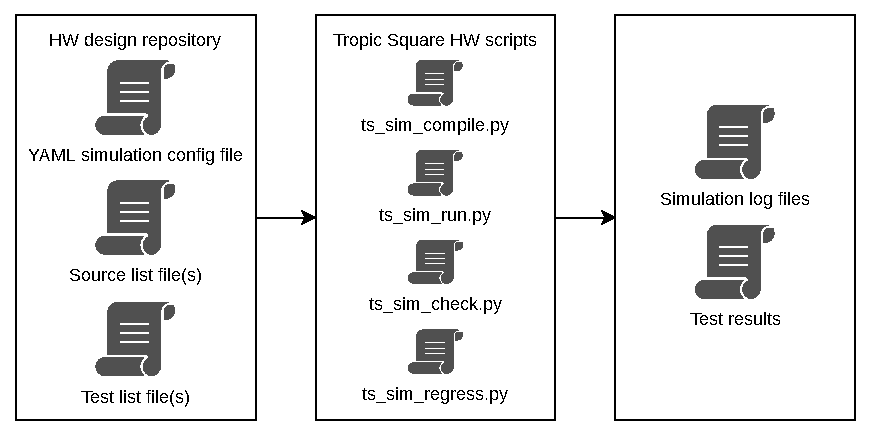
\includegraphics[width=\linewidth]{\detokenize{img/ts_hw_main_block_diagram.pdf}}
    \caption{HW simulation scripting system - Use model}
\end{figure}

Input files (on the left) are HW design repository specific files which configure the
scripting system, allow user to define HDL source files and define tests available
within the repository. These files shall be created by user for each project (see
examples below, "example" folder or "templates" folder in \textit{ts-hw-scripts}
repository).


%%%%%%%%%%%%%%%%%%%%%%%%%%%%%%%%%%%%%%%%%%%%%%%%%%%%%%%%%%%%%%%%%%%%%%%%%%%%%%%%%%%%%%%%%
\subsubsection{Simulation config file}
\label{sec:simulation-config-file}
%%%%%%%%%%%%%%%%%%%%%%%%%%%%%%%%%%%%%%%%%%%%%%%%%%%%%%%%%%%%%%%%%%%%%%%%%%%%%%%%%%%%%%%%%

The simulation config file is a YAML file. It is used to configure HW scripts
and set-up the repository for digital simulation. HW scripting system uses
\textit{\$TS_REPO_ROOT/sim/ts_sim_config.yml} as default simulation config file (it
is possible to override default file by command line switches). If there is no
reasons for choosing alternative path to config file, use default one. If no such
config file exists in repository where you would like to use the scripting system,
either create one (see example below), or copy one from "example" folder of
\textit{ts-hw-scripts} repository. The minimal required content of config file
is as follows:

\begin{lstlisting}
simulator: vcs
test_list_file: <path_to_global_test_list_file>
targets:
    <target_name>:
        top_entity: <name_of_top_entity_for_simulation>
        test_list_file: <path_to_target_specific_test_list_file>
        source_list_files:
            - <path_to_source_list_file>
check_severity: error

\end{lstlisting}

\TropicNote{The example above demonstrates global test list file as well as target
            specific test list file. Only one of these two must be defined (but both
            can be defined).}

Basic keywords within config file have following meaning:

\textbf{simulator} Sets digital simulator, see \ref{sec:how-to-set-simulator}.

\textbf{test_list_file} Points to test list file which defines tests.
    See \ref{sec:test-list-file}.

\textbf{targets} Defines simulation target, its HDL source list file(s) and top entity,
    see \ref{sec:how-to-create-design-target}

\textbf{check_severity} Chooses severity of \textit{ts_sim_check.py} script. See
    \ref{sec:how-to-set-check-severity}.


\TropicNote{
    Relative paths in simulation config file (e.g path to source list files) are always
    interpreted to be relative to \textit{\$TS_REPO_ROOT} environment variable (relative
    to HW design repository root folder). Absolute paths are treated as absolute paths.
}

\TropicNote{
    When scripting system loads simulation config file it throws an error if there are
    invalid keys within config file, there are information missing or there is an
    invalid keyword within the config file. If such an error is thrown, scripting system
    shows you a list of valid keys at position where error occured.
}

\TropicNote{
    Scripting system provides basic set of Error messages which indicate to user when
    something is missing/wrong in config file, or other parts of the scripting system.
    The idea is that the user does not need to dive into details of implementation, but
    works with firmly defined level of abstraction. If you manage to "break" the
    scripting system to such extent, that any of scripts crashes and shows only Python
    stack-trace, please open an issue in \textit{ts-hw-scripts} Gitlab project.
}

\TropicNote{
    Some options specified in simulation scripting flow can be configured also by
    command line switches of scripts. If these options are specified as command line
    switches, they always override the value from simulation config file.
}


%%%%%%%%%%%%%%%%%%%%%%%%%%%%%%%%%%%%%%%%%%%%%%%%%%%%%%%%%%%%%%%%%%%%%%%%%%%%%%%%%%%%%%%%%
\subsubsection{Source list file}
\label{sec:source-list-file}
%%%%%%%%%%%%%%%%%%%%%%%%%%%%%%%%%%%%%%%%%%%%%%%%%%%%%%%%%%%%%%%%%%%%%%%%%%%%%%%%%%%%%%%%%

Source list file is a YAML file which defines HDL sources for compilation/simulation.
Source list files are referenced from simulation config file by filling value for
\textbf{source_list_files} keyword. Source list files are target specific. Source list
files can be nested, see \ref{sec:how-to-point-to-nested-source-list-file} for examples
of nested source list files. A minimal example of source list file content is:

\begin{lstlisting}
library: spi_slave_rtl

source_list:
    - file: spi_tx.vhd
    - file: spi_rx.vhd
    - file: spi_top.dummy_extension
      lang: system_verilog
\end{lstlisting}

This source list file defines 3 source files to be compiled into HDL library
\textbf{spi_slave_rtl}.

\textbf{library} key defines name of HDL library into which the sources will be compiled.
                 See \ref{sec:how-to-define-compilation-library} for more details.

\textbf{source_list} key defines list of source files. A value of this source list
    shall be a YAML list. Each file shall have \textbf{file} keyword with name of
    the HDL file as value.

It is also possible to use the keyword \textbf{lang} to specify the language of the
HDL file, undepending on the file's extension. The current possible values for this
keyword are \textit{vhdl}, \textit{verilog} and \textit{system_verilog}.

\TropicNote{
Relative paths in source list files are interpreted as relative to source list file
itself (not to \textit{\$TS_REPO_ROOT} !). The reason is to allow hierarchical re-use
of source list files across different repositories. Absolute paths are interpreted
as absolute paths.}


%%%%%%%%%%%%%%%%%%%%%%%%%%%%%%%%%%%%%%%%%%%%%%%%%%%%%%%%%%%%%%%%%%%%%%%%%%%%%%%%%%%%%%%%%
\subsubsection{Test list file}
\label{sec:test-list-file}
%%%%%%%%%%%%%%%%%%%%%%%%%%%%%%%%%%%%%%%%%%%%%%%%%%%%%%%%%%%%%%%%%%%%%%%%%%%%%%%%%%%%%%%%%

Test list file is a YAML file which defines tests in current repository.
Test list file is referenced from simulation config file by putting a value to
\textbf{test_list_file} keyword in root of simulation config file, or per-target. Test
list file which is in root, is global for whole repository. Tests from target specific
test list file are available only for a given target. This allows defining different
tests for different targets (if e.g. different target signals different testbench.)
Note that at least one test list file (global or target specific) must be defined.
If none of these two is defined, system throws an error.

Test list files can be nested, see \ref{sec:how-to-point-to-nested-test-list-files}
for details. Tests can be also put into named groups, see
\ref{sec:how-to-define-test-groups} for details. A minimal example of test list file
is following:

\begin{lstlisting}
tests:
    - name: first_test
    - name: second_test
\end{lstlisting}

This example demonstrates definition of two tests: \textit{first_test} and
\textit{second_test}.

\TropicNote{
Relative paths in test list files are interpreted relative to path of test list file
itself (not to \textit{\$TS_REPO_ROOT} !). The reason is to allow hierarchical re-use
of test list files across module/top repositories. Absolute paths are treated as
absolute. Relative paths within test list files are used when specifying nested
test list files.}


%%%%%%%%%%%%%%%%%%%%%%%%%%%%%%%%%%%%%%%%%%%%%%%%%%%%%%%%%%%%%%%%%%%%%%%%%%%%%%%%%%%%%%%%%
\subsubsection{PDK config file}
\label{sec:pdk-config-file}
%%%%%%%%%%%%%%%%%%%%%%%%%%%%%%%%%%%%%%%%%%%%%%%%%%%%%%%%%%%%%%%%%%%%%%%%%%%%%%%%%%%%%%%%%

PDK configuration file is a YAML file which captures information about PDK (Process
development kit). PDK configuration contains:
\begin{itemize}
    \item Definitions of available digital standard cells in the PDK.
    \item Definitions of hard-macros in the PDK.
    \item Definitions of corners available in the PDK.
\end{itemize}

There can be two types of PDK config files:
\begin{itemize}
    \item{Local - Placed in chip top design repository. Typically contains only list of IPs,
                  views and corners used during the design of the chip.}
    \item{Global - Placed in location where PDK is placed. Typically this type of coinfig
                   file contains every IP/standard cell available under given PDK and it
                   is good candidate to be used in IP/Block design repositories for block
                   specific CAD tool setup (e.g. block level synthesis.)} 
\end{itemize}

An example of PDK config file is following:

\begin{lstlisting}[basicstyle=\footnotesize]
name: umc55
corners:
  108c125_wc:
    voltage: 1.08
    temperature: 125
  132c-40_bc:
    voltage: 1.32
    temperature: -40

std_cells:
  - name: umc55uhd
    version: 0.2
    views:
      nldm_db:
        108c125_wc: std_55_UM055LSCEE12BDH/0v2/nldm_db/u055lscee12bdh_108c125_wc.db
        120c25_tc: std_55_UM055LSCEE12BDH/0v2/nldm_db/u055lscee12bdh_120c25_tc.db
        132c-40_bc: std_55_UM055LSCEE12BDH/0v2/nldm_db/u055lscee12bdh_132c-40_bc.db

      gds: std_55_UM055LSCEE12BDH/0v2/gds/u055lscee12bdh.gds
      lef: std_55_UM055LSCEE12BDH/0v2/lef/u055lscee12bdh.lef
      tluplus:
        - std_55_UM055LSCEE12BDH/0v2/tluplus/u055lscee12bdh_RCMAX.TLUPlus
        - std_55_UM055LSCEE12BDH/0v2/tluplus/u055lscee12bdh_RCMIN.TLUPlus
        - std_55_UM055LSCEE12BDH/0v2/map/UMC55_5m0t1f_TLUplus.map
      milkyway: std_55_UM055LSCEE12BDH/0v2/mw
      slf: std_55_UM055LSCEE12BDH/0v2/behav_models/slf_umc55_cells_pg_sdf21.yml

ips:
  - name: flash_UM055EFLLP128KX039S4F
    version: 0.2
    views: 
      lef: ip_55_UM055EFLLP128KX039S4F/0v2/lef/u055efllp128kx039s4f.lef
\end{lstlisting}

The example above defines a PDK with two corners: "108c125_wc" and "132c-40_bc", single
standard cell library "umc55uhd" and single hard macro / IP \newline ("flash_UM055EFLLP128KX039S4F").
Standard cells have "nldm_db", "gds", "lef", "tluplus", "milkyway" and "slf" views defined.
PDK config files support various "views". List of currently supported views can be found
by running \textit{ts_design_cfg.py ----list-supported-views}. Views can be with corner,
or without corner. Views with corner need to have single file defined per corner
defined. Views without corner can define single file, or list of multiple files per view.

Relative paths in PDK config file are interpreted relative to location of PDK config
file itself.

\TropicNote{
    "slf" view of PDK objects shall contain path to source-list file(s) with HDL sources
    for given hard-macro. This is typically used to include simulation models of standard cells
    or hard-macros. Such source list file can be referenced in simulation config file,
    see \ref{sec:how-include-source-list-files-from-pdk}.
}


%%%%%%%%%%%%%%%%%%%%%%%%%%%%%%%%%%%%%%%%%%%%%%%%%%%%%%%%%%%%%%%%%%%%%%%%%%%%%%%%%%%%%%%%%
\subsubsection{Design config file}
\label{sec:design-config-file}
%%%%%%%%%%%%%%%%%%%%%%%%%%%%%%%%%%%%%%%%%%%%%%%%%%%%%%%%%%%%%%%%%%%%%%%%%%%%%%%%%%%%%%%%%

Design config file contains physical design configuration of given chip / HW block.
It loads PDK information from PDK config file via "pdk_configs" keyword.
PDK config file contains:
\begin{itemize}
    \item {Target PDK (must be loaded from PDK config file)}
    \item {Target standard cells (must be in configured PDK)}
    \item {IPs / Hard macros used by the design}
    \item {Design top (by referencing target from simulation config file)}
    \item {Design modes (pairs of: PDK corner + constraint file)}
    \item {Global constraints}
    \item {Design floorplan}
\end{itemize}

\begin{lstlisting}[basicstyle=\footnotesize]
pdk_configs:
  - /projects/tropic01/pdk/umc/ts_pdk_config.yml

design:
  target: rtl_umc55_synth
  pdk: umc55
  std_cells:
    - umc55uhd: 0.2
  constraints:
    - sdc/tassic_top_physical.sdc
  floorplan: floorplan/def/chip_fp_for_synth.def

  ips:
    - flash_UM055EFLLP128KX039S4F: 0.2

  modes:
    - name: func_min
      corner: 132c-40_bc
      constraints: sdc/tassic_top_func.sdc
    - name: func_max
      corner: 108c125_wc
      constraints: sdc/tassic_top_func.sdc
\end{lstlisting}

The example above loads PDK config file located in \newline
\textit{/projects/tropic01/pdk/umc/ts_pdk_config.yml} and loads all PDKs listed in this file.
Further it defines following in for the design:
\begin{itemize}
    \item Design top (target "rtl_umc55_synth" from Simulation config file.)
    \item Target PDK to be "umc55".
    \item Standard cells used to be "umc55uhd", version 0.2.
    \item Global constraint file (common for all modes).
    \item Floorplan file.
    \item IPs / Hard macros used by design: "flash_UM055EFLLP128KX039S4F" version 0.2.
    \item Two modes: "func_min" and "func_max".
\end{itemize}

Paths relative to Design config file are relative to \textit{\$TS_REPO_ROOT} environment
variable. Default location of Design config file in the HW design repository is in:
\textit{cfg/ts_design_cfg.yml}.


%%%%%%%%%%%%%%%%%%%%%%%%%%%%%%%%%%%%%%%%%%%%%%%%%%%%%%%%%%%%%%%%%%%%%%%%%%%%%%%%%%%%%%%%%
\subsection{Compilation / Simulation flow}
\label{sec:compilation-simulation-flow}
%%%%%%%%%%%%%%%%%%%%%%%%%%%%%%%%%%%%%%%%%%%%%%%%%%%%%%%%%%%%%%%%%%%%%%%%%%%%%%%%%%%%%%%%%

After simulation config file, source list files and test list file has been created,
\textit{\$TS_REPO_ROOT} variable is defined and scripts are available in PATH variable,
the simulation flow with Tropic Square HW scripts consists of following steps:
\begin{itemize}
    \item{Compile source files}
    \item{Run test(s)}
    \item{Evaluate results}
\end{itemize}


%%%%%%%%%%%%%%%%%%%%%%%%%%%%%%%%%%%%%%%%%%%%%%%%%%%%%%%%%%%%%%%%%%%%%%%%%%%%%%%%%%%%%%%%%
\subsubsection{Compiling source files}
\label{sec:compiling-source-files}
%%%%%%%%%%%%%%%%%%%%%%%%%%%%%%%%%%%%%%%%%%%%%%%%%%%%%%%%%%%%%%%%%%%%%%%%%%%%%%%%%%%%%%%%%

Source files can be compiled by running:

\begin{lstlisting}
ts_sim_compile.py <target_name>
\end{lstlisting}

Where \textit{<target_name>} is name of a target from simulation config file, e.g.:

\begin{lstlisting}
ts_sim_compile.py rtl
\end{lstlisting}

\TropicNote{
    Targets can be used model type of design being simulated. Typical targets could be
    "tb_rtl", "tb_gate_min", "tb_gate_typ", "tb_gate_max".
}

\TropicNote{
    When naming targets, prefix them with "rtl_" when these targets contain synthesizable
    code and prefix them with "tb_" when these targets contain testbench sources.
}


%%%%%%%%%%%%%%%%%%%%%%%%%%%%%%%%%%%%%%%%%%%%%%%%%%%%%%%%%%%%%%%%%%%%%%%%%%%%%%%%%%%%%%%%%
\subsubsection{Run test(s)}
\label{sec:run-tests}
%%%%%%%%%%%%%%%%%%%%%%%%%%%%%%%%%%%%%%%%%%%%%%%%%%%%%%%%%%%%%%%%%%%%%%%%%%%%%%%%%%%%%%%%%

A test (simulation) can be executed by running:

\begin{lstlisting}
ts_sim_run.py <target_name> <test_name>
\end{lstlisting}

Where \textit{<target_name>} is name of a target from simulation config file and
\textit{<test_name>} is a name of test from test list file, e.g.:

\begin{lstlisting}
ts_sim_run.py rtl first_test
\end{lstlisting}

\TropicNote{
    It is possible to specify multiple tests for single test-run as well as use wild-cards
    to specify test names. Using \textbf{\textbackslash*} as \textit{test_name} will run all
    tests within the repository.
}


%%%%%%%%%%%%%%%%%%%%%%%%%%%%%%%%%%%%%%%%%%%%%%%%%%%%%%%%%%%%%%%%%%%%%%%%%%%%%%%%%%%%%%%%%
\subsubsection{Evaluate test(s) results}
\label{sec:evaluate-test-results}
%%%%%%%%%%%%%%%%%%%%%%%%%%%%%%%%%%%%%%%%%%%%%%%%%%%%%%%%%%%%%%%%%%%%%%%%%%%%%%%%%%%%%%%%%

After running a test, \textit{ts_sim_check.py} script is automatically called and
result of the test is checked and printed to command line. Result of test can be either
\textbf{PASSED} or \textbf{FAILED}.

HW scripts evaluate results of the test based on two indicators:
\begin{itemize}
    \item Simulator exit code - Non-zero exit code causes test to fail
    \item Simulation Log file - Finding error/warning within simulation log
                                file causes test to fail.
    \item Elaboration Log file - Finding error/warning within elaboration log
                                file causes test to fail. A warnings/errors within elaboration
                                log file will be displayed on separate line. Elaboration log
                                file is searched for error only if \textit{check_elab_log} is set
                                to "true" in simulation config file.
\end{itemize}

\textit{ts_sim_check.py} script parses simulation/elaboration log file line by line and
determines if a line shall be classified as an error or warning. A line is classified
as an error/warning when it matches regular expressions defined under
\textbf{error_patterns}/\textbf{warning_patterns} keyword (see
\ref{sec:how-to-classify-errors-warnings-in-elaboration-simulation-output} in simulation
config file.

If there was at least one line from log file classified as Error, test fails.
If there was at least one line classified as Warning and value of
\textbf{check_severity} keyword in simulation config file is set to
\textbf{warning}, test also fails.

\TropicNote{This mechanism for error detection is generic and allows configuring
all kinds of errors types ranging from UVM_ERROR, through analog model errors,
through custom timing violation formats, and it is therefore more flexible than
any purely simulator based error reporting library or framework!}

Each call of \textit{ts_sim_check.py} will export JUnit report in
\textit{\$TS_REPO_ROOT/sim/sim_logs/ts_sim_junit_out.xml}. JUnit output can be
propagated to Gitlab CI by placing \textbf{reports} keyword into \textit{.gitlab-ci.yml}
file like so:

\begin{lstlisting}
artifacts:
name: example_test_results
when: always
paths:
    - sim/sim_logs/ts_sim_junit_out.xml
reports:
    junit: sim/sim_logs/ts_sim_junit_out.xml
\end{lstlisting}

Thanks to the example above, Gitlab will detect \textit{ts-hw-scripts} test results
and natively display them:

\begin{figure}[H]
    \centering
    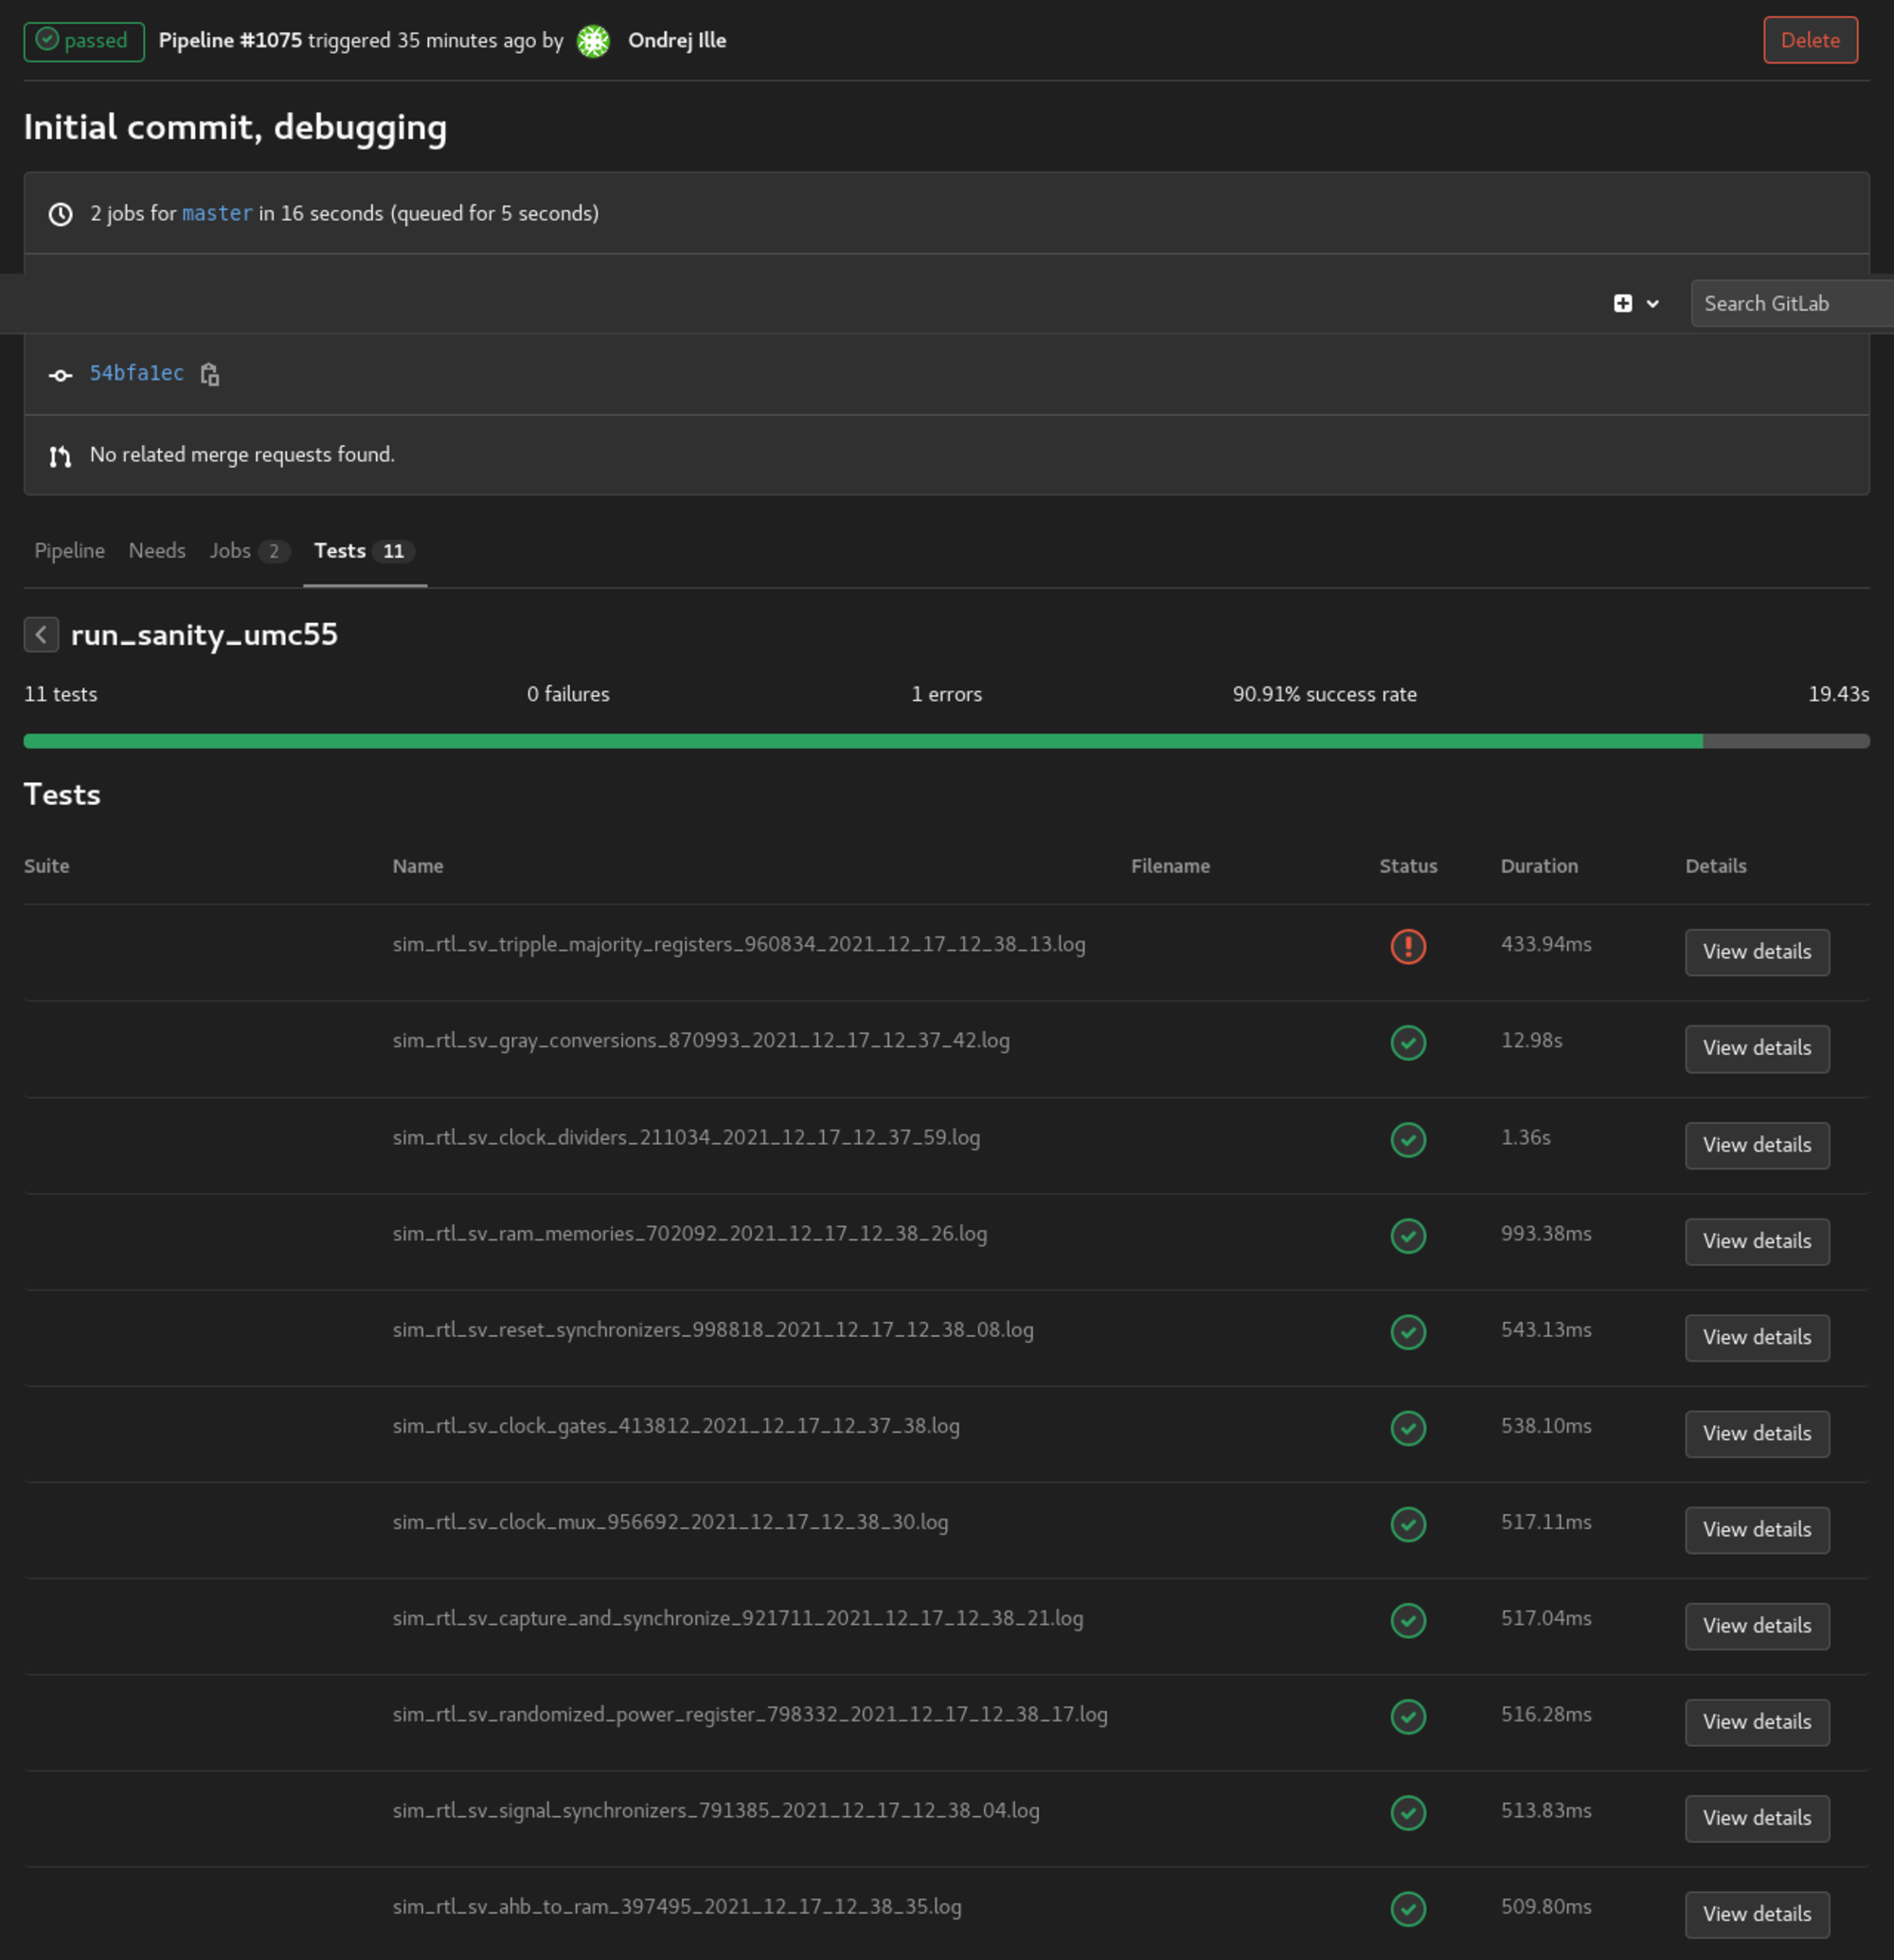
\includegraphics[width=\textwidth]{\detokenize{img/junit_out.pdf}}
\end{figure}


%%%%%%%%%%%%%%%%%%%%%%%%%%%%%%%%%%%%%%%%%%%%%%%%%%%%%%%%%%%%%%%%%%%%%%%%%%%%%%%%%%%%%%%%%
\subsubsection{Running parallel regression}
\label{sec:running-parallel-regression}
%%%%%%%%%%%%%%%%%%%%%%%%%%%%%%%%%%%%%%%%%%%%%%%%%%%%%%%%%%%%%%%%%%%%%%%%%%%%%%%%%%%%%%%%%

Scripting system offers two ways of running tests:
\begin{itemize}
    \item {ts_sim_run.py - Runs single test at a time.}
    \item {ts_sim_regress.py - Can run multiple tests at a time in parallel.}
\end{itemize}

Both scripts read available tests from test list files. To specify number of parallel
jobs, use \textit{--regress-jobs} argument of \textit{ts_sim_regress.py} script.

Both scripts run \textit{ts_sim_check.py} after all tests were executed.

Differences between scripts:

\begin{TropicRatioTable2Col}
    {0.5}                            {0.5}
	{ts_sim_run.py 	                 & ts_sim_regress.py}
     Number of test loops in given
     by \textit{--loop} switch.      & Number of loops is given for each test separately
                                       in test list file by \textit{regress_loops} keyword. \Ttlb

     Runs single simulation at once. & Runs \textit{--regress-jobs} simulations at once.\Ttlb

     Requires \textit{--clear-logs}
     switch to remove log files from
     previous simulations.           & Implicitly clears simulation and elaboration log files
                                       from previous simulations. \Ttlb

     Resulting logs are in
     \textit{sim/sim_logs} and
     \textit{sim/elab_logs} folders. & Resulting logs are backed up into regression directory
                                       under \textit{sim/regression_<time>}. Where <time> is
                                       current time when regression ended. \Ttlb

\end{TropicRatioTable2Col}


%%%%%%%%%%%%%%%%%%%%%%%%%%%%%%%%%%%%%%%%%%%%%%%%%%%%%%%%%%%%%%%%%%%%%%%%%%%%%%%%%%%%%%%%%
\subsubsection{Exporting PDK configuration}
\label{sec:exporting-pdk-configuration}
%%%%%%%%%%%%%%%%%%%%%%%%%%%%%%%%%%%%%%%%%%%%%%%%%%%%%%%%%%%%%%%%%%%%%%%%%%%%%%%%%%%%%%%%%

Design config file and PDK config file contains definitions of hard macros and standard
cells used in the chip / block design. It contains list of views, corners and modes
available for physical design process. Typically, in the physical design process multiple
tools need this information (e.g. timing views are needed by synthesis, PnR and sign-off STA.).

Design and PDK config files serve as single place where this information is defined for
a given block / chip design. To propagate this information into each physical design flow,
\textit{ts-hw-scripts} provide `ts_design_cfg.py` export script which generates TCL file with
variables containing paths to these views.

Example of calling such script is:
\begin{lstlisting}
    ts_design_cfg.py -v --add-views=nldm_db,gds,tluplus
                        --exp-tcl-design-cfg debug.tcl
                        --add-top-entity
                        --add-syn-rtl-build-dirs
                        --add-constraints
                        --add-floorplan    
\end{lstlisting}



%%%%%%%%%%%%%%%%%%%%%%%%%%%%%%%%%%%%%%%%%%%%%%%%%%%%%%%%%%%%%%%%%%%%%%%%%%%%%%%%%%%%%%%%%
\subsection{Directory / file structure}
%%%%%%%%%%%%%%%%%%%%%%%%%%%%%%%%%%%%%%%%%%%%%%%%%%%%%%%%%%%%%%%%%%%%%%%%%%%%%%%%%%%%%%%%%

%%%%%%%%%%%%%%%%%%%%%%%%%%%%%%%%%%%%%%%%%%%%%%%%%%%%%%%%%%%%%%%%%%%%%%%%%%%%%%%%%%%%%%%%%
\subsubsection{Compilation directories}
\label{sec:compilation-directories}
%%%%%%%%%%%%%%%%%%%%%%%%%%%%%%%%%%%%%%%%%%%%%%%%%%%%%%%%%%%%%%%%%%%%%%%%%%%%%%%%%%%%%%%%%

By default, scripting system compiles all HDL files into \textit{\$TS_REPO_ROOT/sim/build}
directory. Each HDL library is compiled to a separate sub-directory within this directory.
It is possible to override compilation directory by command line switches. If
elaboration/simulation creates an executable binary, it is placed to stand-alone
sub-directory of \textit{\$TS_REPO_ROOT/sim/build} directory for each test.


%%%%%%%%%%%%%%%%%%%%%%%%%%%%%%%%%%%%%%%%%%%%%%%%%%%%%%%%%%%%%%%%%%%%%%%%%%%%%%%%%%%%%%%%%
\subsubsection{Log files}
\label{sec:log-files}
%%%%%%%%%%%%%%%%%%%%%%%%%%%%%%%%%%%%%%%%%%%%%%%%%%%%%%%%%%%%%%%%%%%%%%%%%%%%%%%%%%%%%%%%%

Scripting system places compile log files to \textit{\$TS_REPO_ROOT/sim/comp_logs}
directory, elaboration log files to \textit{\$TS_REPO_ROOT/sim/elab_logs} directory
and simulation log files to \textit{\$TS_REPO_ROOT/sim/sim_logs} directory.

When running a test, simulation/elaboration log file contain "sim_"/"elab" prefix in
their name. By default, scripting system appends timestamp to simulation/elaboration
log file. If \textbf{timestamp_log_file} keyword in simulation config file is set to
"false", timestamp is not appended to simulation/elaboration log file.


%%%%%%%%%%%%%%%%%%%%%%%%%%%%%%%%%%%%%%%%%%%%%%%%%%%%%%%%%%%%%%%%%%%%%%%%%%%%%%%%%%%%%%%%%
\subsubsection{Elaboration / Simulation directories}
\label{sec:elaboration-simulation-directories}
%%%%%%%%%%%%%%%%%%%%%%%%%%%%%%%%%%%%%%%%%%%%%%%%%%%%%%%%%%%%%%%%%%%%%%%%%%%%%%%%%%%%%%%%%

Scripting system executes compilation in \textit{\$TS_REPO_ROOT/sim/build} directory
regardless of the location from where you call \textit{ts_sim_compile.py} script. If you
interrupt the compilation process while it is running, it is possible you will end up in
a directory different from the one you launched the compilation from.

Scripting system executes elaboration and simulation from test specific directory under
\textit{\$TS_REPO_ROOT/sim/build}, therefore all simulator specific outputs will be
located in such directory. Each test specific directory is auto-generated, and it
places test name, target name and simulation seed to directory name,
therefore multiple runs of the tests do not overwrite each-another. E.g. when we
run test \textbf{dummy_test} with target \textbf{rtl} and seed 12345, the system will
create directory: \textit{\$TS_REPO_ROOT/sim/build/rtl_dummy_test_12345} and place
all simulator specific files into this directory.


%%%%%%%%%%%%%%%%%%%%%%%%%%%%%%%%%%%%%%%%%%%%%%%%%%%%%%%%%%%%%%%%%%%%%%%%%%%%%%%%%%%%%%%%%
\subsection{Coverage flow}
\label{sec:coverage-flow}
%%%%%%%%%%%%%%%%%%%%%%%%%%%%%%%%%%%%%%%%%%%%%%%%%%%%%%%%%%%%%%%%%%%%%%%%%%%%%%%%%%%%%%%%%

When simulation is run with coverage options enabled, it produces a coverage analysis
database per test. These databases can be merged with the command \textit{ts_sim_coverage.py}.


%%%%%%%%%%%%%%%%%%%%%%%%%%%%%%%%%%%%%%%%%%%%%%%%%%%%%%%%%%%%%%%%%%%%%%%%%%%%%%%%%%%%%%%%%
\subsubsection{Merging coverage databases}
\label{sec:merging-coverage-databases}
%%%%%%%%%%%%%%%%%%%%%%%%%%%%%%%%%%%%%%%%%%%%%%%%%%%%%%%%%%%%%%%%%%%%%%%%%%%%%%%%%%%%%%%%%

Coverage databases can be merged by running:

\begin{lstlisting}
ts_sim_coverage.py <test_dir> [<test_dir>] -o <merged_db>
\end{lstlisting}

As an example:

\begin{lstlisting}
ts_sim_coverage.py rtl_test_2893 rtl_test_5654 -o rtl_test_db
\end{lstlisting}

The script will merge the coverage databases \textit{rtl_test_2893/simv.vdb} and
\textit{test_5654/simv.vdb} into \textit{rtl_test_db.vdb}


\TropicNote{
Input tests directories are relative to \textit{\$TS_REPO_ROOT/\$TS_BUILD_PATH}.
Output database directory is relative to \textit{\$TS_REPO_ROOT/\$TS_COVERAGE_DIR_PATH}.
}


%%%%%%%%%%%%%%%%%%%%%%%%%%%%%%%%%%%%%%%%%%%%%%%%%%%%%%%%%%%%%%%%%%%%%%%%%%%%%%%%%%%%%%%%%
\subsubsection{Visualize merged database}
\label{sec:visualize-merged-database}
%%%%%%%%%%%%%%%%%%%%%%%%%%%%%%%%%%%%%%%%%%%%%%%%%%%%%%%%%%%%%%%%%%%%%%%%%%%%%%%%%%%%%%%%%

It is also possible to watch the content of  the merged database by adding
the \textbf{--gui} option:

\begin{lstlisting}
ts_sim_coverage.py <test_dir> [<test_dir>] -o <merged_db> --gui
\end{lstlisting}

The script will merge the input tests coverage databases and then will open
the output database in a graphical user interface.

\TropicNote{
The current GUI is \textit{DVE}.
}

If the output database already exists, there is no need to specify input tests.

\begin{lstlisting}
ts_sim_coverage.py -o <merged_db> --gui
\end{lstlisting}


%%%%%%%%%%%%%%%%%%%%%%%%%%%%%%%%%%%%%%%%%%%%%%%%%%%%%%%%%%%%%%%%%%%%%%%%%%%%%%%%%%%%%%%%%
% Examples
%%%%%%%%%%%%%%%%%%%%%%%%%%%%%%%%%%%%%%%%%%%%%%%%%%%%%%%%%%%%%%%%%%%%%%%%%%%%%%%%%%%%%%%%%

\subsection{Examples}


%%%%%%%%%%%%%%%%%%%%%%%%%%%%%%%%%%%%%%%%%%%%%%%%%%%%%%%%%%%%%%%%%%%%%%%%%%%%%%%%%%%%%%%%%
\subsubsection{How to set simulator ?}
\label{sec:how-to-set-simulator}
%%%%%%%%%%%%%%%%%%%%%%%%%%%%%%%%%%%%%%%%%%%%%%%%%%%%%%%%%%%%%%%%%%%%%%%%%%%%%%%%%%%%%%%%%

Simulator used by scripting system can be set by \textbf{simulator} keyword in
simulation config file. E.g.:

\begin{lstlisting}
simulator: vcs
\end{lstlisting}

\TropicNote{
\textbf{simulator} keyword is obligatory keyword of simulation config file.
}

\TropicNote{
Currently, VCS is the only supported simulator.
}


%%%%%%%%%%%%%%%%%%%%%%%%%%%%%%%%%%%%%%%%%%%%%%%%%%%%%%%%%%%%%%%%%%%%%%%%%%%%%%%%%%%%%%%%%
\subsubsection{How to create design target ?}
\label{sec:how-to-create-design-target}
%%%%%%%%%%%%%%%%%%%%%%%%%%%%%%%%%%%%%%%%%%%%%%%%%%%%%%%%%%%%%%%%%%%%%%%%%%%%%%%%%%%%%%%%%

Design target can be created by placing an entry under \textbf{targets} keyword in
simulation config file, e.g.:

\begin{lstlisting}
targets:
    rtl:
        top_entity: spi_slave_rtl.spi_top
        source_list_files:
            - rtl/spi_slave_rtl.yml
\end{lstlisting}

The example above creates target \textbf{rtl} with top entity
\textbf{spi_slave_rtl.spi_top}. Note that library name is used as a prefix of top entity.
Target contains source files which are located in
\textit{\$TS_REPO_ROOT/rtl spi_slave_rtl.yml} source list file (assuming default location
of simulation config file).

\TropicNote{
\textbf{top_entity} and \textbf{source_list_files} keywords are obligatory for each
defined target.
}


%%%%%%%%%%%%%%%%%%%%%%%%%%%%%%%%%%%%%%%%%%%%%%%%%%%%%%%%%%%%%%%%%%%%%%%%%%%%%%%%%%%%%%%%%
\subsubsection{How to define compile options?}
\label{sec:how-to-define-compile-options}
%%%%%%%%%%%%%%%%%%%%%%%%%%%%%%%%%%%%%%%%%%%%%%%%%%%%%%%%%%%%%%%%%%%%%%%%%%%%%%%%%%%%%%%%%

Compile options can be defined globally - in the root of the simulation config file -
or can be specific for one target. To do so use the keyword \textbf{comp_options}.
If compilation options are defined in a target, they enrich the eventual compilation
options defined at the root level.

Example:

\begin{lstlisting}
comp_options:
    common: -switch_1
    vcs: -switch_2
targets:
    rtl_0:
        top_entity: rtl_0.top
        source_list_file:
            - slf_0.yml
        comp_options:
            common: -switch_3
            vcs: -switch_4
    rtl_1:
        top_entity: rtl_1.top
        source_list_file:
            - slf_1.yml
\end{lstlisting}

In the example above compiling the target \textbf{rtl_0} with the VCS simulator will use
all the compilation options but only \textit{-switch_1} and \textit{-switch_3}
with another one.
Compiling the target \textbf{rtl_1} with the VCS simulator will use \textit{-switch_1}
and \textit{-switch_2} but only \textit{-switch_1} with another one.

\TropicNote{
The distinction between simulators is unnecessary now, since only VCS is supported,
it is designed for future expandability.
}
\vspace{3mm}

Local compile options (specific to a HDL file, or group of files) can be placed to
source list file, e.g.:

\begin{lstlisting}
library: spi_slave_rtl
comp_options:
    common: -my_fancy_switch

source_list:
    - file: spi_tx.vhd
      comp_options:
        common: -tx_only_switch
    - file: spi_rx.vhd
    - file: spi_top.vhd
\end{lstlisting}

The example above will add \textit{-my_fancy_switch} to compile command when
compiling all files from the source list file, and it will also add
\textit{-tx_only_switch} when compiling \textit{spi_tx.vhd} file.

\TropicNote{
Compile options can be specified global or local, however they can not be specified
test specific (test should not depend on TB/RTL compilation and vice-versa).
}


%%%%%%%%%%%%%%%%%%%%%%%%%%%%%%%%%%%%%%%%%%%%%%%%%%%%%%%%%%%%%%%%%%%%%%%%%%%%%%%%%%%%%%%%%
\subsubsection{How to define compilation library?}
\label{sec:how-to-define-compilation-library}
%%%%%%%%%%%%%%%%%%%%%%%%%%%%%%%%%%%%%%%%%%%%%%%%%%%%%%%%%%%%%%%%%%%%%%%%%%%%%%%%%%%%%%%%%

Compilation library is defined by \textbf{library} keyword in source list file. E.g.:

\begin{lstlisting}
library: spi_slave_rtl

source_list:
    - file: spi_tx.vhd
      comp_options:
        common: -tx_only_switch
    - file: spi_rx.vhd
    - file: spi_top.vhd
    - file: dummy.v
      library: dummy_rtl
\end{lstlisting}

The example above compiles 3 spi_* files to \textbf{spi_slave_rtl} library, and
\textit{dummy.v} file to \textbf{dummy_rtl} library. It is therefore possible to
set file-specific library.

\TropicNote{
A global compilation library is required in each source list file. The scripting system
does not allow relying on default ("work") library.
}


%%%%%%%%%%%%%%%%%%%%%%%%%%%%%%%%%%%%%%%%%%%%%%%%%%%%%%%%%%%%%%%%%%%%%%%%%%%%%%%%%%%%%%%%%
\subsubsection{How to enable UVM?}
\label{sec:how-to-enable-uvm}
%%%%%%%%%%%%%%%%%%%%%%%%%%%%%%%%%%%%%%%%%%%%%%%%%%%%%%%%%%%%%%%%%%%%%%%%%%%%%%%%%%%%%%%%%

To enable UVM (Universal Verification Methodology) for compilation, set \textbf{enable_uvm}
keyword in simulation config file. This will include pre-compiled UVM distribution shipped
with VCS simulator. E.g.:

\begin{lstlisting}
enable_uvm: true
\end{lstlisting}

Note that \textbf{enable_uvm} keyword can be placed in root of simulation config file
or under a target. If placed under a target, UVM compilation is enabled only when
compiling that target. This allows having mixture of UVM/non-UVM testbenches within a
single repository.


%%%%%%%%%%%%%%%%%%%%%%%%%%%%%%%%%%%%%%%%%%%%%%%%%%%%%%%%%%%%%%%%%%%%%%%%%%%%%%%%%%%%%%%%%
\subsubsection{How to define elaboration / simulation options?}
\label{sec:how-to-define-elaboration-simulation-options}
%%%%%%%%%%%%%%%%%%%%%%%%%%%%%%%%%%%%%%%%%%%%%%%%%%%%%%%%%%%%%%%%%%%%%%%%%%%%%%%%%%%%%%%%%

To define elaboration/simulation options use \textbf{elab_options} / \textbf{sim_options}
keywords in simulation config file and/or in test list file. Options will
be appended to elaboration/simulation command issued to a simulator.
Elaboration and/or simulation options shall be defined either at root or at target
level of simulation config file, while test-specific elaboration/simulation options
shall be defined in test list file.
E.g.:

\begin{lstlisting}
elab_options:
    common: -root-common-elab-opt
    vcs: -root-vcs-elab-opt
sim_options:
    common: -root-common-sim-opt
    vcs: -root-vcs-sim-opt
targets:
    rtl_0:
        top_entity: rtl_0.top
        source_list_file:
            - slf_0.yml
        elab_options:
            common: -rtl_0-common-elab-opt
            vcs: -rtl_0-vcs-elab-opt
        sim_options:
            common: -rtl_0-common-sim-opt
            vcs: -rtl_0-vcs-sim-opt
    rtl_1:
        top_entity: rtl_1.top
        source_list_file:
            - slf_1.yml
\end{lstlisting}

In the example above \textit{-root-common-elab-opt} and \textit{-root-common-sim-opt}
will be used in the elaboration and simulation phases respectively on all simulators.
\textit{-root-vcs-elab-opt} and \textit{-root-vcs-sim-opt} will be added if VCS is used.
The options of \textbf{rtl_0} will also be used if tests are run on this target.
\textbf{rtl_1} does not have any target-specific options so only the root options
will be used when running tests on this target.

\begin{lstlisting}
elab_options:
    common: -common-test-switch
tests:
    - name: first_test
      sim_options:
          common: -first-test-only-switch
    - name: second_test
\end{lstlisting}

The example above will add \textit{-common-test-switch} to elaboration command for
both tests and additionally \textit{-first-test-only-switch} to simulation command
when running \textbf{first_test}.


%%%%%%%%%%%%%%%%%%%%%%%%%%%%%%%%%%%%%%%%%%%%%%%%%%%%%%%%%%%%%%%%%%%%%%%%%%%%%%%%%%%%%%%%%
\subsubsection{How to define generics / parameters ?}
\label{sec:how-to-define-generics-parameters}
%%%%%%%%%%%%%%%%%%%%%%%%%%%%%%%%%%%%%%%%%%%%%%%%%%%%%%%%%%%%%%%%%%%%%%%%%%%%%%%%%%%%%%%%%

To define top level generics(VHDL) place them as YAML dictionary under \textbf{generics}
keyword of simulation config file. To define top level parameters (Verilog / System Verilog)
place them as YAML dictionary under \textbf{parameters} keyword of simulation config file.
Note that when you have VHDL top, always use \textbf{generics}, when you have Verilog /
System Verilog, use \textbf{parameters}. E.g.:

\begin{lstlisting}
generics:
    G_MY_INTEGER_GENERIC: 2                 # Integer
    G_MY_STRING_GENERIC: Hello world!       # String
    G_MY_LOGIC_GENERIC: "'0'"               # std_logic
    G_MY_LOGIC_VECT_GENERIC: '"01010101"'   # std_logic_vector
    G_MY_TIME_GENERIC: 25ns                 # time
    G_MY_BOOL_GENERIC: true                 # Boolean
\end{lstlisting}

\begin{lstlisting}
parameters:
    G_MY_INTEGER_PARAMETER: 2           # Integer parameter
    G_MY_STRING_PARAMETER: Hello world! # String
    G_MY_LOGIC_PARAMETER : 1            # Logic parameter
    G_MY_BIT_PARAMETER : 0              # Bit parameter
    G_MY_LOGIC_VECT_PARAMETER : 255     # Logic vector (decimal)
    G_MY_REAL_PARAMETER : 3.14          # Real parameter
    G_MY_TIME_PARAMETER: 25             # Time (multiple of
                                        #       time precision)
\end{lstlisting}

\vspace{0.5cm}

To define test-specific generics/parameters, place \textbf{generics}/\textbf{parameters} keyword
into test  list file. E.g.:

\begin{lstlisting}
tests:
    - name: first_test
      generics:
        G_TEST_NAME: first_test
    - name: second_test
      generics:
        G_TEST_NAME: second_test
\end{lstlisting}

The example above shows how to define test specific generics in test list file. If
test name in TB environment is defined by \textbf{G_TEST_NAME} top level generic,
this example shows how to pass name of the test from scripting system to TB. The
same applies for \textbf{parameters} keyword when having Verilog/System Verilog designs.

\TropicNote{
    The system allows overriding only top level generics, not generics within a
    design hierarchy.
}

\TropicNote{
    When test name is passed to TB (either via generic, or to UVM TB), only its name
    as written in test list file is passed, not the whole name including group prefix!
}


%%%%%%%%%%%%%%%%%%%%%%%%%%%%%%%%%%%%%%%%%%%%%%%%%%%%%%%%%%%%%%%%%%%%%%%%%%%%%%%%%%%%%%%%%
\subsubsection{How to define Verilog / System Verilog macros ?}
\label{sec:how-to-define-verilog-system-verilog-macros}
%%%%%%%%%%%%%%%%%%%%%%%%%%%%%%%%%%%%%%%%%%%%%%%%%%%%%%%%%%%%%%%%%%%%%%%%%%%%%%%%%%%%%%%%%

Macros for Verilog and SystemVerilog HDL files can be defined by \textbf{define} keyword
in simulation config file and source list file(s). To define a global macro (used with
all Verilog/System Verilog files being compiled), place \textbf{define} keyword in root
of simulation config file, e.g.:

\begin{lstlisting}
define:
    MACRO_WITHOUT_VALUE:
    MACRO_WITH_VALUE: 10
\end{lstlisting}

This example defines two macros: \textbf{MACRO_WITHOUT_VALUE} and \textbf{MACRO_WITH_VALUE}
whose value is 10.

To define macro for group of files, place \textbf{define} keyword to root of source list file, e.g.:

\begin{lstlisting}
library: spi_slave_rtl
define:
    MACRO_FOR_ALL_SPI_FILES:

source_list:
    - file: spi_tx.sv
    - file: spi_rx.sv
    - file: spi_top.sv
\end{lstlisting}

The example above will compile 3 files with marco \textbf{MACRO_FOR_ALL_SPI_FILES} defined
only for these 3 files.

Alternatively, it is possible to define file-specific macro by placing \textbf{define}
keyword into definition of source file in source list file

\begin{lstlisting}
library: spi_slave_rtl
source_list:
    - file: spi_tx.sv
    - file: spi_rx.sv
      define:
        MACRO_FOR_SPI_RX
    - file: spi_top.sv
      define:
        MACRO_FOR_SPI_TOP
\end{lstlisting}

The example above defines macro \textbf{MACRO_FOR_SPI_TOP} only in \textit{spi_top.sv}
source file and \textbf{MACRO_FOR_SPI_RX} only in \textit{spi_rx.sv}.

To define per-target specific macros, place \textbf{define} under
target name in simulation config file, e.g.:

\begin{lstlisting}
targets:
    rtl:
        top_entity: my_lib.my_rtl_entity
        define:
            RVFI:
        source_list_files:
            - rtl/src_lst.yml
\end{lstlisting}

The example above will define \textbf{RVFI} macro directory when
compiling all Verilog/System Verilog source files from \textbf{rtl} target.

\TropicNote{
Macros can be defined only for Verilog/System Verilog files. VHDL (until 2019) has
no concept of pre-processor macros, therefore any defined macros are ignored for VHDL
files.
}


%%%%%%%%%%%%%%%%%%%%%%%%%%%%%%%%%%%%%%%%%%%%%%%%%%%%%%%%%%%%%%%%%%%%%%%%%%%%%%%%%%%%%%%%%
\subsubsection{How to define include directories ?}
\label{sec:how-to-define-include-directories}
%%%%%%%%%%%%%%%%%%%%%%%%%%%%%%%%%%%%%%%%%%%%%%%%%%%%%%%%%%%%%%%%%%%%%%%%%%%%%%%%%%%%%%%%%

To define global include directory where simulator will look for Verilog/System
Verilog header files, use \textbf{include_dirs} keyword in root level of simulation config
file, and YAML list of directories as value. E.g.:

\begin{lstlisting}
include_dirs:
    - rtl/include
\end{lstlisting}

The example above will include folder \textit{\$TS_REPO_ROOT/rtl/include} to be searched
for Verilog/System Verilog header files when compiling all Verilog/System Verilog files
(from all targets).

To define include directory for group of files, use \textbf{define} in root of source
list file, e.g.:

\begin{lstlisting}
include_dirs:
    - include

source_list:
    - file: spi_tx.sv
    - file: spi_rx.sv
    - file: spi_top.sv
\end{lstlisting}

The example above will add directory \textit{include} to directories where simulator
will search for header files only for 3 files from this example.

To define per-file specific include directory, use \textbf{include_dirs} as per-file
specific key in source file list, e.g.:

\begin{lstlisting}
library: spi_slave_rtl
source_list:
    - file: spi_tx.sv
      include_dirs:
        - include
    - file: spi_rx.sv
      include_dirs:
        - include
    - file: spi_top.sv
\end{lstlisting}

The example above will add folder \textit{include} when searching for header files
during compilation of \textit{spi_tx.sv} and \textit{spi_rx.sv}, but it will not
search this directory when compiling \textit{spi_top.sv}.

\TropicNote{
Both examples above assume that \textit{include} directory is in the same folder as
source list file itself, since relative paths within source list files are interpreted
as relative to source list file itself.
}

To define per-target specific include directories, place \textbf{include_dirs} under
target name in simulation config file, e.g.:

\begin{lstlisting}
targets:
    rtl:
        top_entity: my_lib.my_rtl_entity
        include_dirs:
            - rtl/include
        source_list_files:
            - rtl/src_lst.yml
\end{lstlisting}

The example above will include \textit{\$TS_REPO_ROOT/rtl/include} directory when
compiling all Verilog/System Verilog source files from \textbf{rtl} target.

\TropicNote{
Include directories are ignored for VHDL files, since VHDL has no concept of header files.
}

%%%%%%%%%%%%%%%%%%%%%%%%%%%%%%%%%%%%%%%%%%%%%%%%%%%%%%%%%%%%%%%%%%%%%%%%%%%%%%%%%%%%%%%%%
\subsubsection{How to increase script verbosity ?}
\label{sec:how-to-increase-script-verbosity}
%%%%%%%%%%%%%%%%%%%%%%%%%%%%%%%%%%%%%%%%%%%%%%%%%%%%%%%%%%%%%%%%%%%%%%%%%%%%%%%%%%%%%%%%%

All scripts in scripting system contain arguments to increase their verbosity. Note that
this only refers to verbosity of the script, not verbosity during simulation. Verbosity
of script can be used to check actual command issued to the simulator.
There are following switches available:
\begin{itemize}
    \item{-v   - Verbose, displays commands being issued}
    \item{-vv  - Very verbose, displays underlying compiler/simulator command}
    \item{-vvv - Debug mode, displays almost all actions executed by the scripts}
\end{itemize}

\begin{lstlisting}
ts_sim_compile.py -v rtl
\end{lstlisting}

The example above will print each compile command to command line before being executed.


%%%%%%%%%%%%%%%%%%%%%%%%%%%%%%%%%%%%%%%%%%%%%%%%%%%%%%%%%%%%%%%%%%%%%%%%%%%%%%%%%%%%%%%%%
\subsubsection{How to point to nested source list files ?}
\label{sec:how-to-point-to-nested-source-list-file}
%%%%%%%%%%%%%%%%%%%%%%%%%%%%%%%%%%%%%%%%%%%%%%%%%%%%%%%%%%%%%%%%%%%%%%%%%%%%%%%%%%%%%%%%%

Source list files can be nested (one source list file can contain a reference to
another source list file). To define nested source list file, use YAML file as
name of the file when listing sources under \textbf{source_list} keyword. Scripting
system will automatically interpret this file as nested source list file and load all
source files from this nested list file. Scripting system recognizes file types based
on file extension according to following rules:

\begin{itemize}
    \item{.vhd     - Recognized as VHDL file, invokes VHDL compiler}
    \item{.v       - Recognized as Verilog file, invokes Verilog compiler}
    \item{.sv      - Recognized as System Verilog file, invokes System Verilog compiler}
    \item{.yml     - Recognized as nested source list file, loads all source files
                     from this list file}
\end{itemize}

\begin{lstlisting}
library: tassic_rtl
source_list:
    - file: spi_slave_rtl.yml
    - file: i2c_slave_rtl.yml
    - file: cpu_rtl.yml
    - file: common_blocks_rtl.yml
    - file: tassic_top.sv
\end{lstlisting}

The example above will load 4 nested list files before loading top source file of
a design. Design library is specified for whole list file, however, nested list
files will contain their own \textbf{library} keyword, therefore overriding top
level library.


%%%%%%%%%%%%%%%%%%%%%%%%%%%%%%%%%%%%%%%%%%%%%%%%%%%%%%%%%%%%%%%%%%%%%%%%%%%%%%%%%%%%%%%%%
\subsubsection{How to list all source files ?}
\label{sec:how-to-list-all-source-files}
%%%%%%%%%%%%%%%%%%%%%%%%%%%%%%%%%%%%%%%%%%%%%%%%%%%%%%%%%%%%%%%%%%%%%%%%%%%%%%%%%%%%%%%%%

To list all source files for a given target, use following switch of
\textit{ts_sim_compile.py}:

\begin{lstlisting}
ts_sim_compile.py --list-sources rtl
\end{lstlisting}

The example above will not compile source files, it will only show flat list
of all source files that shall be compiled for target \textit{rtl}. The source
files will be grouped by compilation library.


%%%%%%%%%%%%%%%%%%%%%%%%%%%%%%%%%%%%%%%%%%%%%%%%%%%%%%%%%%%%%%%%%%%%%%%%%%%%%%%%%%%%%%%%%
\subsubsection{How to point to nested test list files ?}
\label{sec:how-to-point-to-nested-test-list-files}
%%%%%%%%%%%%%%%%%%%%%%%%%%%%%%%%%%%%%%%%%%%%%%%%%%%%%%%%%%%%%%%%%%%%%%%%%%%%%%%%%%%%%%%%%

To define nested test list file, use \textbf{sub_list} key within test list file and
path to nested test list file as value for this key, e.g.:

\begin{lstlisting}
tests:
    - name: first_test
    - name: second_test
    - sub_list: additional_test_list.yml
\end{lstlisting}

The example above will define two tests (\textbf{first_test} and \textbf{second_test})
and enter \textit{additional_test_list.yml} file and load all tests from this file.
Note that nested list file must follow the same syntax as other test list files.
When \textbf{sub_list} keyword is defined within entry of YAML list under \textbf{tests}
keyword, and \textbf{name} keyword is not part of this entry, tests from nested
list file are not added to a test group, but they form a flat list with tests from
original list file.

\TropicNote{
It is obligatory for each list entry in test list file under \textbf{tests} key to
define either \textbf{name} or \textbf{sub_list} keywords. Presence of \textbf{sub_list}
keyword distinguishes between test definition and reference to a nested list file.}


%%%%%%%%%%%%%%%%%%%%%%%%%%%%%%%%%%%%%%%%%%%%%%%%%%%%%%%%%%%%%%%%%%%%%%%%%%%%%%%%%%%%%%%%%
\subsubsection{How to define test groups ?}
\label{sec:how-to-define-test-groups}
%%%%%%%%%%%%%%%%%%%%%%%%%%%%%%%%%%%%%%%%%%%%%%%%%%%%%%%%%%%%%%%%%%%%%%%%%%%%%%%%%%%%%%%%%

Tests can be divided into groups to avoid naming conflicts when having many tests.
Only tests from nested list file (see \ref{sec:how-to-point-to-nested-test-list-files})
can be placed into test group. When tests are placed into a group, their name is
prefixed with group name. When running a test from group by \textit{ts_sim_run.py},
you need to provide full test name including group name (effectively test name is
extended with group name). E.g.:

\begin{lstlisting}
tests:
    - name: first_test
    - name: second_test
    - sub_list: additional_test_list.yml
      name: test_group_a
\end{lstlisting}

The example above places all tests from \textit{additional_test_list.yml} test list
file into test group "test_group_a". If we assume that there are two tests
\textbf{test_red} and \textbf{test_green} defined in \textit{additional_test_list.yml},
the above configuration will define following tests:

\begin{itemize}
    \item{first_test}
    \item{second_test}
    \item{test_group_a.test_red}
    \item{test_group_a.test_green}
\end{itemize}

\TropicNote{
    Due to wild-card support in \textit{ts_sim_run.py} it is easy to run all tests
    from a group by using group name and * when specifying tests to be executed.
}

\TropicNote{
    It is possible to place tests from multiple test list files into single group.
    To do this, just define multiple the same test group multiple times with different
    test list file. Tests from this file will be appended to previously defined tests
    in the group.
}

%%%%%%%%%%%%%%%%%%%%%%%%%%%%%%%%%%%%%%%%%%%%%%%%%%%%%%%%%%%%%%%%%%%%%%%%%%%%%%%%%%%%%%%%%
\subsubsection{How to list all available tests ?}
\label{sec:how-to-list-all-available-tests}
%%%%%%%%%%%%%%%%%%%%%%%%%%%%%%%%%%%%%%%%%%%%%%%%%%%%%%%%%%%%%%%%%%%%%%%%%%%%%%%%%%%%%%%%%

To list all tests within a repository, use \textit{--list-tests} switch of
\textit{ts_sim_run.py}:

\begin{lstlisting}
ts_sim_run.py --list-tests rtl
\end{lstlisting}

The example above will not run any tests, it will only list tests available
for execution.


%%%%%%%%%%%%%%%%%%%%%%%%%%%%%%%%%%%%%%%%%%%%%%%%%%%%%%%%%%%%%%%%%%%%%%%%%%%%%%%%%%%%%%%%%
\subsubsection{How to run all tests ?}
\label{sec:how-to-run-all-tests}
%%%%%%%%%%%%%%%%%%%%%%%%%%%%%%%%%%%%%%%%%%%%%%%%%%%%%%%%%%%%%%%%%%%%%%%%%%%%%%%%%%%%%%%%%

To run all tests, on needs to pass escape linux wild-card identifier (*) when passing name
of the test to \textit{ts_sim_run.py}:

\begin{lstlisting}
    ts_sim_run.py rtl \*
\end{lstlisting}


%%%%%%%%%%%%%%%%%%%%%%%%%%%%%%%%%%%%%%%%%%%%%%%%%%%%%%%%%%%%%%%%%%%%%%%%%%%%%%%%%%%%%%%%%
\subsubsection{How to pass Test name to testbench ?}
\label{sec:how-to-pass-test-name-to-testbench}
%%%%%%%%%%%%%%%%%%%%%%%%%%%%%%%%%%%%%%%%%%%%%%%%%%%%%%%%%%%%%%%%%%%%%%%%%%%%%%%%%%%%%%%%%

Typically, names of tests defined in test list files need to be passed to TB. This can
be done either manually, by specifying \textbf{generics} / \textbf{parameters} for each
entry in test list file, or by specifying test name strategy.

There are two test name strategies available:
\begin{itemize}
    \item generic/parameter
    \item uvm
\end{itemize}

Test name passing strategy is set by \textbf{test_name_strategy} in root of simulation
config file, e.g.:

\begin{lstlisting}
test_name_strategy: uvm
\end{lstlisting}

The example above will pass name of each test from all loaded test list files (including
test group prefix) to UVM TB environment.

When using "generic/parameter" strategy, top level generic / parameter will be set to test name. It
is designer's/verifier's responsibility to implement such string generic on top level
entity/module which is being simulated. E.g.:

\begin{lstlisting}
test_name_strategy: generic_parameter
test_name_generic: G_TEST_NAME
\end{lstlisting}

The example above will set top level generic G_TEST_NAME to name of each test executed.
When \textbf{test_name_strategy}=generic, \textbf{test_name_generic} keyword is obligatory
in root of simulation config file.

Note that \textbf{test_name_strategy} keyword can be placed in root of simulation config
file, or under a target. If placed under a target, then test name will be passed to
simulation only when running it with given target.


%%%%%%%%%%%%%%%%%%%%%%%%%%%%%%%%%%%%%%%%%%%%%%%%%%%%%%%%%%%%%%%%%%%%%%%%%%%%%%%%%%%%%%%%%
\subsubsection{How to randomize simulation / define seed ?}
\label{sec:how-to-randomize-simulation-define-seed}
%%%%%%%%%%%%%%%%%%%%%%%%%%%%%%%%%%%%%%%%%%%%%%%%%%%%%%%%%%%%%%%%%%%%%%%%%%%%%%%%%%%%%%%%%

By default (if no seed is specified), random seed is generated, therefore simulation
is randomized. To specify seed, use \textbf{seed} keyword in root level of simulation
config file, e.g.:

\begin{lstlisting}
seed: 150
\end{lstlisting}

or use \textit{--seed} switch of \textit{ts_sim_run.py} script like so:

\begin{lstlisting}
ts_sim_run.py --seed 150 rtl first_test
\end{lstlisting}

Both of the examples above will set seed to 150 for simulation.


%%%%%%%%%%%%%%%%%%%%%%%%%%%%%%%%%%%%%%%%%%%%%%%%%%%%%%%%%%%%%%%%%%%%%%%%%%%%%%%%%%%%%%%%%
\subsubsection{How to debug simulation in GUI ?}
\label{sec:how-to-debug-simulation-in-gui}
%%%%%%%%%%%%%%%%%%%%%%%%%%%%%%%%%%%%%%%%%%%%%%%%%%%%%%%%%%%%%%%%%%%%%%%%%%%%%%%%%%%%%%%%%

To run simulation in GUI, use \textit{--gui} switch of \textit{ts_sim_run.py} script.
It is possible to use either \textbf{dve}, \textbf{verdi} as wiever, \textbf{dve} being
the default choice if no viewer is specified.

\begin{lstlisting}
ts_sim_run.py --gui rtl first_test
ts_sim_run.py --gui=dve rtl first_test
ts_sim_run.py --gui verdi rtl first_test
\end{lstlisting}

The example above will launch interactive simulation with \textit{DVE} as GUI in the
first two cases and with \textit{Verdi} in the third case.

\TropicNote{
Using \textit{--gui} options will not record the whole waveform hierarchy by default.
}


%%%%%%%%%%%%%%%%%%%%%%%%%%%%%%%%%%%%%%%%%%%%%%%%%%%%%%%%%%%%%%%%%%%%%%%%%%%%%%%%%%%%%%%%%
\subsubsection{How to restore simulation GUI with loaded waveforms ?}
\label{sec:how-to-restore-simulation-gui-with-loaded-waveforms}
%%%%%%%%%%%%%%%%%%%%%%%%%%%%%%%%%%%%%%%%%%%%%%%%%%%%%%%%%%%%%%%%%%%%%%%%%%%%%%%%%%%%%%%%%

To restore waveforms, when launching simulation with GUI, you can pass "session file"
to \textit{--session-file} option of \textit{ts_sim_run.py}.

\begin{lstlisting}
ts_sim_run.py --gui --session-file=my_session.tcl rtl first_test
\end{lstlisting}

The example will launch an interactive simulation and load session file \textit{my_session.tcl}.

The meaning of session files is simulator specific:

\begin{TropicRatioTable3Col}
    {0.2}             {0.2}               {0.6}
	{Simulator 	    & Waveform viewer 	& Session file}
        VCS         & DVE               & TCL Session file obtained in DVE GUI by "File->Save session". \Ttlb
\end{TropicRatioTable3Col}


%%%%%%%%%%%%%%%%%%%%%%%%%%%%%%%%%%%%%%%%%%%%%%%%%%%%%%%%%%%%%%%%%%%%%%%%%%%%%%%%%%%%%%%%%
\subsubsection{How to log all waveform hierarchy ?}
\label{sec:how-to-log-all-waveform-hierarchy}
%%%%%%%%%%%%%%%%%%%%%%%%%%%%%%%%%%%%%%%%%%%%%%%%%%%%%%%%%%%%%%%%%%%%%%%%%%%%%%%%%%%%%%%%%

To dump waveform database from whole design hierarchy, use \textit{--dump-waves}
option of \textit{ts_sim_run.py} script like so:

\begin{lstlisting}
ts_sim_run.py --dump-waves rtl first_test
\end{lstlisting}

\TropicNote{\textit{--dump-waves} switch is intended to be used together with
\textit{--gui} to dump whole hierarchy for subsequent analysis in waveform viewer.
}

\TropicNote{
Waveform hierarchy database is simulator specific and it is always dumped to
test specific sub-folder under \textit{\$TS_REPO_ROOT/sim/build} directory.
Currently, VCS uses "VDB" database format.
}


%%%%%%%%%%%%%%%%%%%%%%%%%%%%%%%%%%%%%%%%%%%%%%%%%%%%%%%%%%%%%%%%%%%%%%%%%%%%%%%%%%%%%%%%%
\subsubsection{How run single test multiple times ?}
\label{sec:how-to-run-single-test-multiple-times}
%%%%%%%%%%%%%%%%%%%%%%%%%%%%%%%%%%%%%%%%%%%%%%%%%%%%%%%%%%%%%%%%%%%%%%%%%%%%%%%%%%%%%%%%%

To run single test multiple times, use \textit{--loop} option of \textit{ts_sim_run.py} script like so:

\begin{lstlisting}
ts_sim_run.py --loop 10 rtl first_test
\end{lstlisting}

The example above will run \textbf{first_test} 10 times. If no seed is specified,
a random seed will be generated for each run.


%%%%%%%%%%%%%%%%%%%%%%%%%%%%%%%%%%%%%%%%%%%%%%%%%%%%%%%%%%%%%%%%%%%%%%%%%%%%%%%%%%%%%%%%%
\subsubsection{How run multiple tests ?}
\label{sec:how-to-run-multiple-tests}
%%%%%%%%%%%%%%%%%%%%%%%%%%%%%%%%%%%%%%%%%%%%%%%%%%%%%%%%%%%%%%%%%%%%%%%%%%%%%%%%%%%%%%%%%

Let's assume we have following tests defined in test list file:

\begin{lstlisting}
tests:
    - name: spi_tx_test
    - name: spi_rx_test
    - name: spi_err_test
\end{lstlisting}

To run all tests at once you can either pass the name of all the tests as arguments of
\textit{ts_sim_run.py} like so:

\begin{lstlisting}
ts_sim_run.py rtl spi_tx_test spi_rx_test spi_err_test
\end{lstlisting}

or use Linux-like wildcards to run all the tests matching a "spi_" prefix like so:

\begin{lstlisting}
ts_sim_run.py rtl spi_*
\end{lstlisting}

The behavior of both examples above is equivalent, in each case 3 tests will be
executed.


%%%%%%%%%%%%%%%%%%%%%%%%%%%%%%%%%%%%%%%%%%%%%%%%%%%%%%%%%%%%%%%%%%%%%%%%%%%%%%%%%%%%%%%%%
\subsubsection{How to disable colored output ?}
\label{sec:how-to-disable-colored-output}
%%%%%%%%%%%%%%%%%%%%%%%%%%%%%%%%%%%%%%%%%%%%%%%%%%%%%%%%%%%%%%%%%%%%%%%%%%%%%%%%%%%%%%%%%

By default HW scripts use colors when printing to standard output. This approach
allows quickly spotting important parts of script output. However, this option
might be inconvenient when running in a shell environments which do not support
ANSI coloring. To disable colored output, use \textit{--no-color} switch like so:

\begin{lstlisting}
ts_sim_run.py --no-color rtl first_test
\end{lstlisting}


%%%%%%%%%%%%%%%%%%%%%%%%%%%%%%%%%%%%%%%%%%%%%%%%%%%%%%%%%%%%%%%%%%%%%%%%%%%%%%%%%%%%%%%%%
\subsubsection{How to disable simulation output to terminal ?}
\label{sec:how-to-disable-simulation-output-to-terminal}
%%%%%%%%%%%%%%%%%%%%%%%%%%%%%%%%%%%%%%%%%%%%%%%%%%%%%%%%%%%%%%%%%%%%%%%%%%%%%%%%%%%%%%%%%

By default, HW scripts print simulation and elaboration log to standard output and also
to test specific log files. This is useful for debugging, however in CI environment,
it is unnecessary and might cause job log overflow. To disable elaboration
and simulation output to standard output, use \textit{--no-sim-out} option
of \textit{ts_sim_run.py} script like so:

\begin{lstlisting}
ts_sim_run.py --no-sim-out rtl first_test
\end{lstlisting}


%%%%%%%%%%%%%%%%%%%%%%%%%%%%%%%%%%%%%%%%%%%%%%%%%%%%%%%%%%%%%%%%%%%%%%%%%%%%%%%%%%%%%%%%%
\subsubsection{How to run only elaboration ?}
\label{sec:how-to-run-only-elaboration}
%%%%%%%%%%%%%%%%%%%%%%%%%%%%%%%%%%%%%%%%%%%%%%%%%%%%%%%%%%%%%%%%%%%%%%%%%%%%%%%%%%%%%%%%%

By default, \textit{ts_sim_run.py} runs elaboration and simulation together by single
run of the script. To perform only elaboration, use \textit{--elab-only} option of
\textit{ts_sim_run.py} script like so:

\begin{lstlisting}
ts_sim_run.py --elab-only rtl first_test
\end{lstlisting}


%%%%%%%%%%%%%%%%%%%%%%%%%%%%%%%%%%%%%%%%%%%%%%%%%%%%%%%%%%%%%%%%%%%%%%%%%%%%%%%%%%%%%%%%%
\subsubsection{How to run only simulation ?}
\label{sec:how-to-run-only-simulation}
%%%%%%%%%%%%%%%%%%%%%%%%%%%%%%%%%%%%%%%%%%%%%%%%%%%%%%%%%%%%%%%%%%%%%%%%%%%%%%%%%%%%%%%%%

It is also possible to run only the simulation using the \textit{--sim-only} option of
\textit{ts_sim_run.py} script like so:

\begin{lstlisting}
ts_sim_run.py --sim-only rtl first_test
\end{lstlisting}

Please note that the elaboration phase will not be run if this option is activated, so
make sure your design is elaborated beforehand.


%%%%%%%%%%%%%%%%%%%%%%%%%%%%%%%%%%%%%%%%%%%%%%%%%%%%%%%%%%%%%%%%%%%%%%%%%%%%%%%%%%%%%%%%%
\subsubsection{How to queue for simulation license ?}
\label{sec:how-to-queue-for-simulation-license}
%%%%%%%%%%%%%%%%%%%%%%%%%%%%%%%%%%%%%%%%%%%%%%%%%%%%%%%%%%%%%%%%%%%%%%%%%%%%%%%%%%%%%%%%%

By default, when simulation is executed and simulator fails to obtain a license,
\textit{ts_sim_run.py} quits. To enable polling for license, use \textit{--license-wait}
switch of \textit{ts_sim_run.py} script like so:

\begin{lstlisting}
ts_sim_run.py --license-wait rtl first_test
\end{lstlisting}

Alternatively, you can configure \textbf{license_wait} keyword and set its value to
"true" in root level of simulation config file, like so:

\begin{lstlisting}
license_wait: true
\end{lstlisting}


%%%%%%%%%%%%%%%%%%%%%%%%%%%%%%%%%%%%%%%%%%%%%%%%%%%%%%%%%%%%%%%%%%%%%%%%%%%%%%%%%%%%%%%%%
\subsubsection{How to classify errors / warnings in elaboration/simulation output ?}
\label{sec:how-to-classify-errors-warnings-in-elaboration-simulation-output}
%%%%%%%%%%%%%%%%%%%%%%%%%%%%%%%%%%%%%%%%%%%%%%%%%%%%%%%%%%%%%%%%%%%%%%%%%%%%%%%%%%%%%%%%%

\textit{ts_sim_check.py} script parses simulation/elaboration log file line after line and classifies
whether a line is a warning or an error. A line is classified as a warning if it matches a
regular expression listed under \textbf{warning_patterns} keyword in simulation config
file. Similarly, a line is classified as an error if it matches a regular expression
listed under \textbf{error_patterns} keyword in simulation config file. Note that it is
possible to configure "common" patterns which cause failure under all simulators, and
simulator specific patterns.

\begin{lstlisting}
error_patterns:
    common:
        - 'My fancy error'
    vcs:
        - 'Totally broken in VCS...'

warning_patterns:
    common:
        - 'Important warning'
    vcs:
        - 'VCS specific warning'
\end{lstlisting}

The example above shows an example configuration which can classify UVM_ERRORs/ UVM_WARNINGs
as errors/warnings by \textit{ts_sim_check.py} script. This example also shows VCS specific
patterns which match format of log caused by VHDLs "report <MESSAGE> severity error/warning"
in VCS simulator.

Apart from user defined errors/warning, there are common patterns which always cause
a line to be classified as an error/warning. Common error patterns are:
\begin{itemize}
    \item {Occurrence of string \textbf{UVM_ERROR} or \textbf{UVM_FATAL}}
    \item {A log entry caused by \$error, \$fatal (Verilog), or report <msg> severity
           error/failure (VHDL)}
    \item {Log entry caused by VHDL PSL / SVA assertion failure.}
    \item {Timing violation caused by standard cell libraries}
\end{itemize}

Common warning patterns are:
\begin{itemize}
    \item {Occurrence of string \textbf{UVM_WARNING}}
    \item {A log entry caused by \$warning (Verilog), or report <msg> severity warning (VHDL)}
\end{itemize}

\TropicNote{The distinction between common and simulator specific patterns is unnecessary
now since scripting system only supports VCS simulator, it is however important for future
extensions since different simulators can have different format of error reports (e.g.
Cadence has "E*: <message>" for report with error severity.)
}


%%%%%%%%%%%%%%%%%%%%%%%%%%%%%%%%%%%%%%%%%%%%%%%%%%%%%%%%%%%%%%%%%%%%%%%%%%%%%%%%%%%%%%%%%
\subsubsection{How to check also elaboration log file ?}
\label{sec:how-to-check-also-elaboration-log}
%%%%%%%%%%%%%%%%%%%%%%%%%%%%%%%%%%%%%%%%%%%%%%%%%%%%%%%%%%%%%%%%%%%%%%%%%%%%%%%%%%%%%%%%%

By default, scripting system only parses simulation log file for error and warning patterns.
When \textbf{check_elab_log} is set, scripting system parses also elaboration log file
for errors/warning patterns. E.g.:

\begin{lstlisting}
    check_elab_log: true
\end{lstlisting}

Note that when showing results in test summary, simulation and elaboration log files are
shown as separate entries (on separate lines). Thus, if you run 10 tests, then 20 lines
will be shown in resulting summary.


%%%%%%%%%%%%%%%%%%%%%%%%%%%%%%%%%%%%%%%%%%%%%%%%%%%%%%%%%%%%%%%%%%%%%%%%%%%%%%%%%%%%%%%%%
\subsubsection{How to set check severity ?}
\label{sec:how-to-set-check-severity}
%%%%%%%%%%%%%%%%%%%%%%%%%%%%%%%%%%%%%%%%%%%%%%%%%%%%%%%%%%%%%%%%%%%%%%%%%%%%%%%%%%%%%%%%%

Check severity is configured by the \textbf{check_severity} keyword in simulator config file.
It has to be one of the following values: \textbf{error} or \textbf{warning}. When check
severity is set to "warning", lines from simulation/elaboration log file classified as Warnings or
Errors cause test failure. When check severity is set to "error" only lines which are
classified as Errors cause test failure. E.g.:

\begin{lstlisting}
check_severity: warning
\end{lstlisting}


%%%%%%%%%%%%%%%%%%%%%%%%%%%%%%%%%%%%%%%%%%%%%%%%%%%%%%%%%%%%%%%%%%%%%%%%%%%%%%%%%%%%%%%%%
\subsubsection{How to signal end of simulation?}
\label{sec:how-to-signal-end-of-simulation}
%%%%%%%%%%%%%%%%%%%%%%%%%%%%%%%%%%%%%%%%%%%%%%%%%%%%%%%%%%%%%%%%%%%%%%%%%%%%%%%%%%%%%%%%%

If simulation is aborted (e.g. CTRL+C), then it is often desirable to mark the test
as failed even if no error has occurred yet. To do this, the testbench needs to print
a special phrase when regularly exiting simulation and configure this phrase as value
of \textbf{post_sim_msg} keyword in simulation config file. If this phrase is not found
in simulation log file, test will be marked as failed regardless of 0 found errors/warnings.

If \textbf{post_sim_msg} keyword is not defined, check for this keyword is not executed.

\begin{lstlisting}
post_sim_msg: TS_TB_ENDING_OK
\end{lstlisting}

The example above will fail any test unless 'TS_TB_ENDING_OK' is found in simulation
log file.


%%%%%%%%%%%%%%%%%%%%%%%%%%%%%%%%%%%%%%%%%%%%%%%%%%%%%%%%%%%%%%%%%%%%%%%%%%%%%%%%%%%%%%%%%
\subsubsection{How to ignore errors / warnings ?}
\label{sec:how-to-ignore-errors-warnings}
%%%%%%%%%%%%%%%%%%%%%%%%%%%%%%%%%%%%%%%%%%%%%%%%%%%%%%%%%%%%%%%%%%%%%%%%%%%%%%%%%%%%%%%%%

It is possible that certain errors in simulation log occur, and they can't be debugged or
fixed. If these errors are not a functional issue, they should not cause tests to fail,
and these errors can be ignored. A typical example are timing violations occuring in
timing gate level simulations upon POR assertion at start of simulation.

Errors/Warnings can be ignored by configuring \textbf{error_ignore_start}/
\textbf{warning_ignore_start} and \textbf{error_ignore_stop}/\textbf{warning_ignore_stop}
keywords in simulation config file. Errors/Warnings which are ignored does not cause
test to fail.

If \textit{ts_sim_check.py} matches \textbf{error_ignore_start}/\textbf{warning_ignore_start}
pattern on a line of simulation/elaboration log file, it will ignore all errors/warnings
until it matches \textbf{error_ignore_stop}/\textbf{warning_ignore_stop} on another line
of simulation log file. E.g.

\begin{lstlisting}
error_ignore_start: 'TS_ERR_IGNORE_START'
error_ignore_stop: 'TS_ERR_IGNORE_STOP'
error_ignore_start: 'TS_WARN_IGNORE_START'
error_ignore_stop: 'TS_WARN_IGNORE_STOP'
\end{lstlisting}

The example above specifies two patterns which can be used to ignore errors/warnings.
If TB prints these patterns into simulation/elaboration log file in correct simulation time (e.g.
just before POR assertion), then this mechanism can be used to safely ignore errors.

\TropicNote {
It is the responsibility of the developer not to ignore any real functional errors,
only false positives.
}

\TropicNote{
If \textit{ts_sim_check.py} starts ignoring errors/warnings because it encounters
\textbf{error_ignore_start}/\textbf{warning_ignore_start} pattern, then it must also
encounter the \textbf{error_ignore_stop}/\textbf{warning_ignore_stop} before the end
of simulation/elaboration log file. If it does not find it, the test will fail regardless of
number of non-ignored errors.
}

%%%%%%%%%%%%%%%%%%%%%%%%%%%%%%%%%%%%%%%%%%%%%%%%%%%%%%%%%%%%%%%%%%%%%%%%%%%%%%%%%%%%%%%%%
\subsubsection{How to call other scripts ?}
\label{sec:how-to-call-other-scripts}
%%%%%%%%%%%%%%%%%%%%%%%%%%%%%%%%%%%%%%%%%%%%%%%%%%%%%%%%%%%%%%%%%%%%%%%%%%%%%%%%%%%%%%%%%

Third-party scripts can be embedded into simulation scripting flow by means of hooks.
A hook is a callback which is called at a specific time during the compilation/simulation process.
Hooks can be configured in simulation config file (global hooks), or in test list file
(test specific hooks). Each hook is defined as a path to an executable script (hook is
sourced by scripting flow) or as a bash command. A hook is defined by placing one of
the following keywords to the simulation config file and/or the test list file:
\begin{itemize}
    \item {\textbf{pre_compile_hook}}
    \item {\textbf{post_compile_hook}}
    \item {\textbf{pre_run_hook}}
    \item {\textbf{pre_test_hook}}
    \item {\textbf{pre_sim_hook}}
    \item {\textbf{post_test_hook}}
    \item {\textbf{post_run_hook}}
    \item {\textbf{post_check_hook}}
\end{itemize}

An example of global hook (in simulation config file) that will be executed before
each simulation run:

\begin{lstlisting}
pre_run_hook: compile_sw_sources.sh
\end{lstlisting}

In the example above, \textit{compile_sw_sources.sh} script will be called each time
\textit{ts_sim_run.py} is launched.

An example of test-specific hook (in test list file):

\begin{lstlisting}
tests:
    - name: first_test
      pre_test_hook: script.sh
    - name: second_test
      post_test_hook: echo "HELLO WORLD"
    - name: third_test
\end{lstlisting}

In the example above, \textit{script.sh} will be called before starting elaboration of
\textbf{first_test} test, and "HELLO WORLD" will be printed to terminal after
simulation of \textbf{second_test}.

The overall hook flow is following:

\begin{figure}[H]
    \centering
    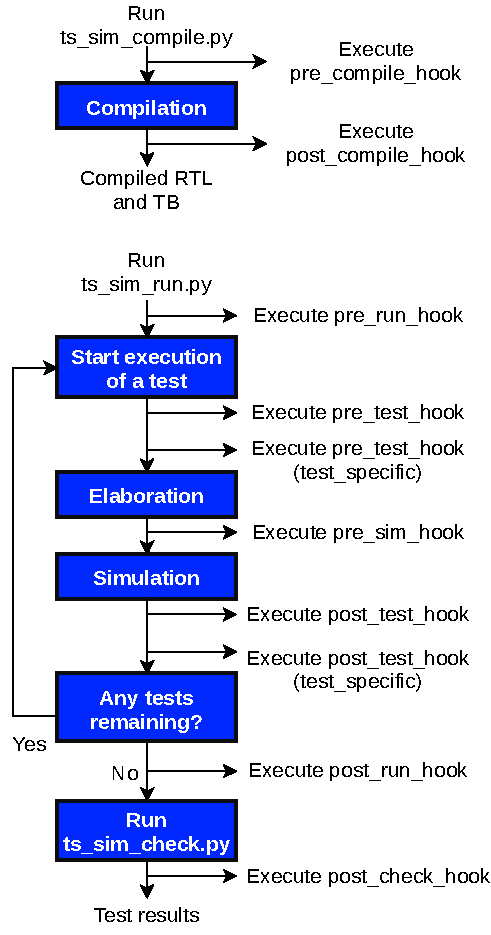
\includegraphics{\detokenize{img/ts_hw_hook_flow.pdf}}
    \caption{Hook flow}
\end{figure}

\TropicNote{
    When scripting system is executing a bash script as a hook, it passes
    3 arguments to pre-test/post-test hooks:
    \begin{itemize}
        \item{Test name}
        \item{Test seed}
        \item{Test loop index}
    \end{itemize}

    These can be accessed within hook script as input arguments (\$1, \$2, \$3)
    and can be used to e.g. perform generation of seed-deterministic data within
    a hook, or choosing different input data for test.

    When hook is specified as a bash command, these arguments are not passed to the command.
}


%%%%%%%%%%%%%%%%%%%%%%%%%%%%%%%%%%%%%%%%%%%%%%%%%%%%%%%%%%%%%%%%%%%%%%%%%%%%%%%%%%%%%%%%%
\subsubsection{How to stop simulating on failed test ?}
\label{sec:how-to-stop-simulating-on-failed-test}
%%%%%%%%%%%%%%%%%%%%%%%%%%%%%%%%%%%%%%%%%%%%%%%%%%%%%%%%%%%%%%%%%%%%%%%%%%%%%%%%%%%%%%%%%

By default, \textit{ts_sim_run.py} runs all tests which are given on command line. If a
test fails, then \textit{ts_sim_run.py} proceeds to the next one. If it is needed to stop
execution of \textit{ts_sim_run.py} after first failed test, use \textit{--fail-fast}
switch of \textit{ts_sim_run.py} script, e.g.:

\begin{lstlisting}
ts_sim_run.py --fail-fast rtl *
\end{lstlisting}

The example above will run all tests within a repository, but it will abort after first
failed test.


%%%%%%%%%%%%%%%%%%%%%%%%%%%%%%%%%%%%%%%%%%%%%%%%%%%%%%%%%%%%%%%%%%%%%%%%%%%%%%%%%%%%%%%%%
\subsubsection{How to define simulation verbosity ?}
\label{sec:how-to-define-simulation-verbosity}
%%%%%%%%%%%%%%%%%%%%%%%%%%%%%%%%%%%%%%%%%%%%%%%%%%%%%%%%%%%%%%%%%%%%%%%%%%%%%%%%%%%%%%%%%

Simulation verbosity can be defined by setting value for \textbf{sim_verbosity} key in
simulation config file. Valid values for simulation verbosity must be one of:

\begin{itemize}
    \item{debug - Should be used to display all messages.}
    \item{info - Should hide Debug messages.}
    \item{warning - Should hide Debug and Info messages.}
    \item{error - Should hide Debug, Info and Warning messages.}
\end{itemize}

Further, level which is chosen must be defined in \textbf{sim_verbosity_levels} keyword.
When verbosity level is defined, it is up to the user to define how will be this verbosity
level passed to simulator (generics/parameters, elaboration or simulation options). E.g:

\begin{lstlisting}
sim_verbosity_levels:
    info:
        elab_options:
            vcs: "-time_resolution 1ps"
        sim_options:
            common: "-sva -xlrm"
        generics:
            - G_VERBOSITY: info
        parameters:
            - BUS_WIDTH: 16

sim_verbosity: info
\end{lstlisting}

The example above shows that \textbf{elab_options} and \textbf{sim_options} are valid
keywords when defining verbosity level and they can be used similarly as
when specifying global elaboration/simulation options.
The example also shows that verbosity level "info" will set top-level generic
\textbf{G_VERBOSITY} to "info" when running simulation, and it also sets simulation
verbosity within scripting system to "info" level.

\TropicNote{Simulation verbosity mechanism is a generic form of defining simulation
verbosities and translating them to simulator specific verbosity levels (e.g. it is
possible to connect verbosity levels to "UVM verbosity").
}


%%%%%%%%%%%%%%%%%%%%%%%%%%%%%%%%%%%%%%%%%%%%%%%%%%%%%%%%%%%%%%%%%%%%%%%%%%%%%%%%%%%%%%%%%
\subsubsection{How to set language versions ?}
\label{sec:how-to-set-language-versions}
%%%%%%%%%%%%%%%%%%%%%%%%%%%%%%%%%%%%%%%%%%%%%%%%%%%%%%%%%%%%%%%%%%%%%%%%%%%%%%%%%%%%%%%%%

VHDL language version used by underlying simulator is set by \textbf{vhdl_std} key
in simulation config file. Valid values are: \textbf{vhdl87}, \textbf{vhdl93},
\textbf{vhdl02}, \textbf{vhdl08}. Verilog language version is set by \textbf{verilog_std},
valid values are \textbf{v95}, \textbf{v01} and \textbf{v05}.

SystemVerilog language version is not set by any keywords, since VCS does not distinguish
between 2005/2012 and 2017 versions.


%%%%%%%%%%%%%%%%%%%%%%%%%%%%%%%%%%%%%%%%%%%%%%%%%%%%%%%%%%%%%%%%%%%%%%%%%%%%%%%%%%%%%%%%%
\subsubsection{How to set simulation resolution ?}
\label{sec:how-to-set-simulation-resolution}
%%%%%%%%%%%%%%%%%%%%%%%%%%%%%%%%%%%%%%%%%%%%%%%%%%%%%%%%%%%%%%%%%%%%%%%%%%%%%%%%%%%%%%%%%

Simulation resolution of underlying simulator is set by \textbf{simulation_resolution}
keyword in root of simulation config file. This will set simulation resolution for all
targets/tests (target/test specific resolution is not supported). If mixed language
design is present, this will set the resolution and precision for Verilog as well as
VHDL designs. E.g:

\begin{lstlisting}
simulation_resolution: fs
\end{lstlisting}

The example above will set simulation resolution / precision to 1fs / 1fs.

\TropicNote{
    Supported values are: \textbf{fs}, \textbf{ps}, \textbf{ns}, \textbf{us},
        \textbf{ms}, \textbf{s}.
}


%%%%%%%%%%%%%%%%%%%%%%%%%%%%%%%%%%%%%%%%%%%%%%%%%%%%%%%%%%%%%%%%%%%%%%%%%%%%%%%%%%%%%%%%%
\subsubsection{How to force recompilation of all sources ?}
\label{sec:how-to-force-recompilation-of-all-sources?}
%%%%%%%%%%%%%%%%%%%%%%%%%%%%%%%%%%%%%%%%%%%%%%%%%%%%%%%%%%%%%%%%%%%%%%%%%%%%%%%%%%%%%%%%%

If \textit{ts_sim_compile.py} has been previously called, then next calls of this script
will make use of incremental compilation. To force recompilation of all source files,
use \textit{--clear} option of \textit{ts_sim_run.py}. E.g.:

\begin{lstlisting}
ts_sim_compile.py --clear rtl
\end{lstlisting}

The example above will delete the build directory before starting the compilation,
therefore forcing clean-table compilation.


%%%%%%%%%%%%%%%%%%%%%%%%%%%%%%%%%%%%%%%%%%%%%%%%%%%%%%%%%%%%%%%%%%%%%%%%%%%%%%%%%%%%%%%%%
\subsubsection{How to clear log files ?}
\label{sec:how-to-clear-log-files}
%%%%%%%%%%%%%%%%%%%%%%%%%%%%%%%%%%%%%%%%%%%%%%%%%%%%%%%%%%%%%%%%%%%%%%%%%%%%%%%%%%%%%%%%%

To clear log files, use \textit{--clear-logs} switch of \textit{ts_sim_compile.py} or
\textit{ts_sim_run.py} scripts. Using this switch with \textit{ts_sim_compile.py} will
erase all logs from \textit{\$TS_REPO_ROOT/sim/comp_logs} folder. Using this switch with
\textit{ts_sim_compile.py} will erase all logs from \textit{\$TS_REPO_ROOT/sim/elab_logs}
and \textit{\$TS_REPO_ROOT/sim/sim_logs} folders.


%%%%%%%%%%%%%%%%%%%%%%%%%%%%%%%%%%%%%%%%%%%%%%%%%%%%%%%%%%%%%%%%%%%%%%%%%%%%%%%%%%%%%%%%%
\subsubsection{How to show errors/warnings from the test?}
\label{sec:how-to-show-errors-warningsf-from-the-test}
%%%%%%%%%%%%%%%%%%%%%%%%%%%%%%%%%%%%%%%%%%%%%%%%%%%%%%%%%%%%%%%%%%%%%%%%%%%%%%%%%%%%%%%%%

To show simulation/elaboration log file lines which were classified as warnings/errors by
\textit{ts_sim_check.py} script, use \textit{-v} (verbose) option. When running
\textit{ts_sim_run.py} with \textit{-v} option, the subsequent call to
\textit{ts_sim_check.py} will display list of all detected and ignored errors/warnings.


%%%%%%%%%%%%%%%%%%%%%%%%%%%%%%%%%%%%%%%%%%%%%%%%%%%%%%%%%%%%%%%%%%%%%%%%%%%%%%%%%%%%%%%%%
\subsubsection{How to check result of previous test run ?}
\label{sec:how-to-check-result-of-previous-test-run}
%%%%%%%%%%%%%%%%%%%%%%%%%%%%%%%%%%%%%%%%%%%%%%%%%%%%%%%%%%%%%%%%%%%%%%%%%%%%%%%%%%%%%%%%%

\textit{ts_sim_run.py} automatically calls \textit{ts_sim_check.py} after it ends. Check
of test results can be executed manually by user by providing log file path. E.g.

\begin{lstlisting}
ts_sim_check.py sim/sim_logs/*
\end{lstlisting}

The example above will check results of all tests which were run (all log files in
\textit{sim_logs} will be checked).


%%%%%%%%%%%%%%%%%%%%%%%%%%%%%%%%%%%%%%%%%%%%%%%%%%%%%%%%%%%%%%%%%%%%%%%%%%%%%%%%%%%%%%%%%
\subsubsection{How to reference files from simulation?}
\label{sec:how-to-reference-files-from-simulation}
%%%%%%%%%%%%%%%%%%%%%%%%%%%%%%%%%%%%%%%%%%%%%%%%%%%%%%%%%%%%%%%%%%%%%%%%%%%%%%%%%%%%%%%%%

\textit{ts_sim_run.py} creates simulation executable in
\textit{\$TS_REPO_ROOT/sim/build/<target_name>_<test_name>_<seed>} when it runs simulation.
Simulation is also executed from this directory. Consider the following example:

\vspace{0.5cm}

There is \textbf{code.hex} file located in \textit{\$TS_REPO_ROOT/tb/hex_files}. Path to
this file needs to be passed to TB, so that TB can load this file. Passing path to this
file to top level TB entity can be done like so:

\begin{lstlisting}
    entity my_tb_top is
    GENERIC (
        hex_file_path : string := "../../../tb/hex_files/code.hex"
    );
    end entity;
\end{lstlisting}

\TropicNote{"../../.." moves back via \textit{build}, \textit{sim} up to \textit{\$TS_REPO_ROOT}
            directory.}


%%%%%%%%%%%%%%%%%%%%%%%%%%%%%%%%%%%%%%%%%%%%%%%%%%%%%%%%%%%%%%%%%%%%%%%%%%%%%%%%%%%%%%%%%
\subsubsection{How to simulate in "single-step" flow ?}
\label{sec:how-to-simulate-in-single-step-flow}
%%%%%%%%%%%%%%%%%%%%%%%%%%%%%%%%%%%%%%%%%%%%%%%%%%%%%%%%%%%%%%%%%%%%%%%%%%%%%%%%%%%%%%%%%

Typical use-case is to first call \textit{ts_sim_compile.py} and then call {ts_sim_run.py}.
If there is a need to execute these two steps at once, it is possible to use so called
"single-step" flow. This can be done by using \textit{--recompile} switch of
\textit{ts-sim-compile.py}, e.g.:

\begin{lstlisting}
ts_sim_run.py --recompile <target_name> <test_name>
\end{lstlisting}

The above command is equivalent of calling \textit{ts_sim_compile.py --clear rtl} followed
by calling \textit{ts_sim_run.py <target_name> <test_name>}.

If you want to recompile always, set \textbf{recompile} keyword to "true" in root of your
simulation config file, e.g.:

\begin{lstlisting}
recompile: true
\end{lstlisting}


%%%%%%%%%%%%%%%%%%%%%%%%%%%%%%%%%%%%%%%%%%%%%%%%%%%%%%%%%%%%%%%%%%%%%%%%%%%%%%%%%%%%%%%%%
\subsubsection{How to propagate RTL sources to synthesis ?}
\label{sec:how-to-propagate-rtl-sources-to-synthesis}
%%%%%%%%%%%%%%%%%%%%%%%%%%%%%%%%%%%%%%%%%%%%%%%%%%%%%%%%%%%%%%%%%%%%%%%%%%%%%%%%%%%%%%%%%

When doing synthesis, list of sources can be dumped per target. This implies that RTL
codes need to be part of separate target, while testbench target will contain RTL as
well as testbench codes.

To export codes for DC shell/Vivado synthesis, use either \textit{--exp-tcl-file-dc} or
\textit{--exp-tcl-file-vivado} switch of \textit{ts_sim_compile.py}.
When this switch is set, compilation is not executed (nor pre-compile/post-compile
hooks are called), only a TCL script is exported.
This script performs tool specific file commands which load source files from specified
target to synthesis tool. This script is intended to be sourced by a synthesis tool. E.g.

\begin{lstlisting}
ts_sim_compile.py --exp-tcl-file-dc my_block_src.tcl rtl
\end{lstlisting}

The example above will export all source files from \textit{rtl} target to \textit{my_block_src.tcl}
file. When this file is sourced from DC-shell TCL, it will load all source files from \textit{rtl}
target for synthesis.

\TropicNote{Only Vivado and DC shell outputs are supported.}


%%%%%%%%%%%%%%%%%%%%%%%%%%%%%%%%%%%%%%%%%%%%%%%%%%%%%%%%%%%%%%%%%%%%%%%%%%%%%%%%%%%%%%%%%
\subsubsection{How to set number of test repetitions in regression run?}
\label{sec:how-to-set-number-of-repetitions-in-regression-run}
%%%%%%%%%%%%%%%%%%%%%%%%%%%%%%%%%%%%%%%%%%%%%%%%%%%%%%%%%%%%%%%%%%%%%%%%%%%%%%%%%%%%%%%%%

When running parallel regression via \textit{ts_sim_regress.py}, each test can be
repeated N times. N can be different for each test. To do this, use \textbf{regress_loops}
keyword for a test entry in test list file. If number of repetitions is not specified,
then test will run only once. E.g.:

\begin{lstlisting}
tests:
    - name: first_test
    - name: second_test
      regress_loops: 10
    - name: third_test
\end{lstlisting}

In the example above, "second_test" will run 10 times. "first_test" and "third_test" will
run only once.

\TropicNote{
    \textit{ts_sim_run.py} ignores \textbf{regress_loops} keyword, it is only interpreted
    by \textit{ts_sim_regress.py}.
}


%%%%%%%%%%%%%%%%%%%%%%%%%%%%%%%%%%%%%%%%%%%%%%%%%%%%%%%%%%%%%%%%%%%%%%%%%%%%%%%%%%%%%%%%%
\subsubsection{How to number of parallel jobs in regression ?}
\label{sec:how-to-set-number-of-parallel-jobs-in-regression}
%%%%%%%%%%%%%%%%%%%%%%%%%%%%%%%%%%%%%%%%%%%%%%%%%%%%%%%%%%%%%%%%%%%%%%%%%%%%%%%%%%%%%%%%%

Number of parallel jobs in regression can be set by \textit{--regress-jobs} switch of
\textit{ts_sim_regress.py} script. E.g.:

\begin{lstlisting}
ts_sim_regress.py --regress-jobs 3 rtl \*
\end{lstlisting}

The example above will run all defined tests with 3 simulations in parallel.


%%%%%%%%%%%%%%%%%%%%%%%%%%%%%%%%%%%%%%%%%%%%%%%%%%%%%%%%%%%%%%%%%%%%%%%%%%%%%%%%%%%%%%%%%
\subsubsection{How to stop the simulation on message severity ?}
\label{sec:how-to-stop-the-simulation-on-message-severity}
%%%%%%%%%%%%%%%%%%%%%%%%%%%%%%%%%%%%%%%%%%%%%%%%%%%%%%%%%%%%%%%%%%%%%%%%%%%%%%%%%%%%%%%%%

The flow provides the possibility to stop the simulation once a message with a specific
severity is detected by the simulator. The supported values are \textbf{note},
\textbf{warning}, \textbf{error}, \textbf{failure} and \textbf{nostop}. E.g.:

\begin{lstlisting}
stop_severity: warning
\end{lstlisting}

The example above stop the simulation as soon as a message with severity
\textit{warning} is detected.


%%%%%%%%%%%%%%%%%%%%%%%%%%%%%%%%%%%%%%%%%%%%%%%%%%%%%%%%%%%%%%%%%%%%%%%%%%%%%%%%%%%%%%%%%
\subsubsection{How to include the sources of a target in another?}
\label{sec:how-to-include-the-sources-of-a-target-in-another}
%%%%%%%%%%%%%%%%%%%%%%%%%%%%%%%%%%%%%%%%%%%%%%%%%%%%%%%%%%%%%%%%%%%%%%%%%%%%%%%%%%%%%%%%%

Sometimes several targets share the same source files. In this case, maintaining a
consistent list of files for each target quickly become cumbersome as the number of
targets rises. To keep the simulation configuration file light and easy to read, it is
possible to provide a target name in the source list files of another target so the
latter can include the source list files of the former.

The syntax is as follows:
\begin{lstlisting}
targets:
    targetA:
        source_list_files:
            - <targetA source list files>
    targetB:
        source_list_files:
            - <targetA>
            - <targetB source list files>
\end{lstlisting}

\textbf{targetB} will include the source list files of \textbf{targetA} in its own list.

Let's have a look at the example below:
\begin{lstlisting}
targets:
    rtl_0:
        top_entity: my_lib.rtl_0_entity
        source_list_files:
            - rtl/src_lst_rtl_0.yml
    rtl_1:
        top_entity: my_lib.rtl_1_entity
        source_list_files:
            - rtl_0
            - rtl/src_lst_rtl_1.yml
    rtl_2:
        top_entity: my_lib.rtl_2_entity
        source_list_files:
            - rtl_1
            - rtl/src_lst_rtl_2.yml
\end{lstlisting}

In the example above, the target \textbf{rtl_0} contains the file \textit{rtl/src_lst_rtl_0.yml}
as source list file whereas \textbf{rtl_1} contains \textit{rtl/src_lst_rtl_1.yml} \textbf{and}
\textit{rtl/src_lst_rtl_0.yml}. The target \textbf{rtl_2} contains all the three files
\textit{rtl/src_lst_rtl_0.yml}, \textit{rtl/src_lst_rtl_1.yml} and
\textit{rtl/src_lst_rtl_2.yml}.


%%%%%%%%%%%%%%%%%%%%%%%%%%%%%%%%%%%%%%%%%%%%%%%%%%%%%%%%%%%%%%%%%%%%%%%%%%%%%%%%%%%%%%%%%
\subsubsection{How to inherit the configuration of another target?}
\label{sec:how-to-inherit-the-configuration-of-another-target}
%%%%%%%%%%%%%%%%%%%%%%%%%%%%%%%%%%%%%%%%%%%%%%%%%%%%%%%%%%%%%%%%%%%%%%%%%%%%%%%%%%%%%%%%%

Sometimes several targets share more than only the source files and it might be
beneficial to create a target based on another.
To this end it is possible to use the keyword \textbf{inherits}.

Example:
\begin{lstlisting}
targets:
    targetA:
        top_entity: <targetA top entity>
        test_name_strategy: <targetA test name strategy>
        enable_uvm: <targetA enable uvm>
        test_list_file: <targetA test list file>
        source_list_files:
            - <targetA source list files>
        define:
            VAR_A: <VALUE_A>
            VAR_C:
        elab_options:
            vcs: <optsA>
    targetB:
        inherits: targetA
        source_list_files:
            - <targetB source list files>
        define:
            VAR_B: <VALUE_B>
        elab_options:
            vcs: <optsB>
\end{lstlisting}

is equivalent to:

\begin{lstlisting}
targets:
    targetA:
        top_entity: <targetA top entity>
        test_name_strategy: <targetA test name strategy>
        enable_uvm: <targetA enable uvm>
        test_list_file: <targetA test list file>
        source_list_files:
            - <targetA source list files>
        define:
            VAR_A: <VALUE_A>
            VAR_C:
        elab_options:
            vcs: <optsA>

    targetB:
        top_entity: <targetA top entity>
        test_name_strategy: <targetA test name strategy>
        enable_uvm: <targetA enable uvm>
        test_list_file: <targetA test list file>
        source_list_files:
            - <targetA source list files>
            - <targetB source list files>
        define:
            VAR_A: <VALUE_A>
            VAR_C:
            VAR_B: <VALUE_B>
        elab_options:
            vcs: <optsB>
\end{lstlisting}


%%%%%%%%%%%%%%%%%%%%%%%%%%%%%%%%%%%%%%%%%%%%%%%%%%%%%%%%%%%%%%%%%%%%%%%%%%%%%%%%%%%%%%%%%
\subsubsection{How to customize simulation process?}
\label{sec:how-to-customize-simulation-process}
%%%%%%%%%%%%%%%%%%%%%%%%%%%%%%%%%%%%%%%%%%%%%%%%%%%%%%%%%%%%%%%%%%%%%%%%%%%%%%%%%%%%%%%%%

To change the way a simulation is run, you can pass a custom "do" file to
\textit{ts_sim_run.py} and \textit{ts_sim_regress.py} via the option \textit{--do-file}.

\begin{lstlisting}
ts_sim_run.py --do-file=my_do_file rtl first_test
\end{lstlisting}

The example above will launch the simulation and execute the commands from the "do" file.


%%%%%%%%%%%%%%%%%%%%%%%%%%%%%%%%%%%%%%%%%%%%%%%%%%%%%%%%%%%%%%%%%%%%%%%%%%%%%%%%%%%%%%%%%
\subsubsection{How to include source list files from PDK ?}
\label{sec:how-include-source-list-files-from-pdk}
%%%%%%%%%%%%%%%%%%%%%%%%%%%%%%%%%%%%%%%%%%%%%%%%%%%%%%%%%%%%%%%%%%%%%%%%%%%%%%%%%%%%%%%%%

Since PDK config file contains "slf" (source list file) views (typically with
simulation models of hard-macros or standard cells), such models are typically
used in simulation. To reference "slf" view of a an IP / Standard cell defined in
PDK config file, you can use ":" notation when defining source list file for a target
within simulation config file as shown in following example:

\begin{lstlisting}
    targets:
    targetA:
        top_entity: <targetA top entity>
        source_list_files:
            - :umc55uhd:slf_umc55_cells_pg_sdf21.yml

\end{lstlisting}

The example above will attempt to load \textit{slf_umc55_cells_pg_sdf21.yml} from "umc55uhd"
object in current PDK. Current PDK must be loaded in Design config file, and set by
"pdk" keyword under "design" keyword. Path to \textit{slf_umc55_cells_pg_sdf21.yml} must be
listed under "slf" keyword of PDK object (standard cells or an IP) "umc55uhd".
Example of such PDK config file containing "slf" view for "umc55uhd" standard cells
is in \ref{sec:pdk-config-file}.

\TropicNote{
    If multiple PDKs are loaded, only sources from target PDK as configured in "pdk"
    keyword under "design" keyword of PDK config file can be included.
}

\TropicNote{
    Even path in "slf" view of PDK config file contains multiple directories, you only
    need to refer to the name of final source list file. This is to facilitate easy
    switching between versions of hard-macros.
}


%%%%%%%%%%%%%%%%%%%%%%%%%%%%%%%%%%%%%%%%%%%%%%%%%%%%%%%%%%%%%%%%%%%%%%%%%%%%%%%%%%%%%%%%%
% Open issues
%%%%%%%%%%%%%%%%%%%%%%%%%%%%%%%%%%%%%%%%%%%%%%%%%%%%%%%%%%%%%%%%%%%%%%%%%%%%%%%%%%%%%%%%%
\pagebreak
\section{Open Issues}

\PrintOpenIssueSummary

\end{document}
